
    \chapter{Implementação e Evolução Técnica}

    \section{Stack Tecnológica e Metodologias}
    O \textbf{OmniAI SDK} foi desenvolvido em Kotlin Multiplatform \cite{kmp_ref} com targets JVM e JavaScript/Node.js. A escolha de KMP permite partilhar o domínio, os contratos, as portas, os adapters principais e parte da lógica geral entre plataformas, mantendo implementações específicas quando o ambiente o exige \cite{kotlin_multiplatform}. A serialização dos contratos é baseada em Kotlinx Serialization \cite{serialization_ref}, o que facilita a definição explícita dos modelos JSON estudados.

    O \textit{core} do \textbf{OmniAI SDK} é estritamente agnóstico em relação a \textit{frameworks} web e mecanismos de transporte HTTP. Contudo, para fornecer uma solução imediatamente utilizável, o projeto inclui módulos oficiais de integração baseados na \textit{framework} Ktor \cite{ktor_ref}. Estes módulos opcionais oferecem implementações de referência tanto para a execução de pedidos aos fornecedores (\textit{client-side}) como para a exposição das rotas da Gateway (\textit{server-side}). A \textbf{OmniAI Gateway} instanciada como Prova de Conceito (PoC) tira partido destas implementações prontas a usar. No entanto, a adoção do SDK não obriga ao uso do Ktor; a arquitetura garante que qualquer utilizador possa descartar estes módulos e implementar os adaptadores de rede utilizando a tecnologia da sua preferência, como o ecossistema Spring por exemplo, entre outros.

    As ferramentas de desenvolvimento incluíram Git, IntelliJ IDEA, o cliente HTTP do IDE para pedidos REST, Docker Compose para Logto \cite{logto_docs}, PostgreSQL \cite{postgresql_ref}, OpenTelemetry Collector \cite{opentelemetry_what_is}, Prometheus \cite{prometheus_ref} e Grafana \cite{grafana_ref}, além de clientes reais como Claude Code e SDKs oficiais dos fornecedores. Também foram usados assistentes de apoio, como Gemini no browser e agentes de programação como o Antigravity e Codex, para pesquisa, comparação de documentação e aceleração de tarefas, mantendo a validação no código, nos testes e nos cenários executados. Foi criada uma pipeline de \textbf{Continuous Integration} (CI) \cite{CI_ref}    existente executa \texttt{./gradlew clean build} como passo evolutivo, está prevista a criação de uma pipeline de \textbf{Continuous Deployment} (CD) para publicar as versões do nosso Software Development Kit,o \textbf{OmniAI SDK} em Maven e NPM.

    \section{A Primeira Iteração da Gateway}

    A primeira iteração do projeto consistiu numa Gateway HTTP construída diretamente, responsável por receber pedidos de clientes e encaminhá-los para fornecedores de inferência. Esta fase foi útil para validar rapidamente a viabilidade da solução, testar pedidos reais e compreender diferenças práticas entre as diferentes API's dos fornecedores, neste caso da OpenAI \cite{openai_api}, Anthropic\cite{anthropic_api} e Gemini\cite{google_gemini_api}.

    À medida que o sistema cresceu, essa abordagem revelou acoplamento excessivo. A tradução entre contratos, a configuração dos fornecedores, a autenticação, o tratamento de erros e o encaminhamento de pedidos começaram a concentrar-se na própria aplicação. Cada novo fornecedor ou preocupação exigia alterações no mesmo conjunto de componentes, tornando o código difícil de evoluir e de se testar.

A reorganização da arquitetura separou o produto principal, o \textbf{OmniAI SDK}, de uma aplicação final denominada \textbf{OmniAI Gateway}.
O \textbf{OmniAI SDK} passou a concentrar toda a lógica e abstrações reutilizáveis do domínio, incluindo contratos, portas e adaptadores (\textit{Ports \& Adapters}), o sistema de \textit{dispatching}, a \textit{pipeline} de execução, \textit{interceptors}, DSLs de configuração e abstrações HTTP multiplataforma. Desta forma, o SDK fornece toda a infraestrutura necessária para que qualquer utilizador consiga instanciar e configurar a sua própria \textbf{OmniAI Gateway}, adaptada ao seu contexto e necessidades.
A \textbf{OmniAI Gateway} representa, assim, uma aplicação concreta construída sobre o \textbf{OmniAI SDK}. No contexto deste projeto, foi desenvolvida uma \textbf{OmniAI Gateway} responsável por carregar configurações, instanciar os componentes necessários, instalar os conectores Ktor e expor \textit{endpoints} HTTP.

Esta aplicação tem como objetivo validar a arquitetura proposta e demonstrar que o \textbf{OmniAI SDK} permite construir \textit{gateways} funcionais, extensíveis e desacopladas dos diferentes fornecedores de modelos de IA. Assim, a \textbf{OmniAI Gateway} desenvolvida neste projeto atua como uma \textit{Proof of Concept} da abordagem arquitetural definida, servindo como exemplo prático da utilização do SDK.

Esta separação também influenciou o desenho da arquitetura para suportar escalamento horizontal. O \textbf{OmniAI SDK} foi projetado para manter o estado associado aos pedidos apenas em estruturas transitórias, como \texttt{GatewayContext} e \texttt{TypedMap}, expondo portas explícitas para componentes que necessitam de estado partilhado, como \textit{caches}, \textit{rate limiting}, \textit{circuit breakers}, autenticação e observabilidade.

Esta abordagem permite que uma instanciação simples de uma \textbf{OmniAI Gateway} utilize implementações em memória, reduzindo a complexidade inicial de configuração e execução. No entanto, em cenários de escalamento horizontal, esses mesmos mecanismos podem ser substituídos por sistemas distribuídos e partilhados, sem necessidade de alterações nos \textit{inbounds}, \textit{outbounds} ou contratos expostos pelo SDK.

Desta forma, o \textbf{OmniAI SDK} desacopla a lógica funcional da infraestrutura de persistência e sincronização, permitindo que diferentes implementações da \textbf{OmniAI Gateway} evoluam de ambientes locais e monolíticos para arquiteturas distribuídas de forma transparente.

\section{Decisões de Desenho e Alternativas Descartadas}

A análise de \textit{trade-offs} partiu de três critérios principais: preservar a estabilidade da versão demonstrável, manter o \textbf{OmniAI SDK} reutilizável e extensível independentemente da aplicação final e evitar que funcionalidades experimentais introduzissem acoplamento excessivo no domínio comum.

Neste contexto, importa recordar que a \textbf{OmniAI Gateway} apresentada neste projeto corresponde apenas a uma instanciação concreta construída sobre o \textbf{OmniAI SDK}. Assim, várias decisões arquiteturais foram tomadas não apenas a pensar na \textit{Proof of Concept}, mas sobretudo na preservação do SDK enquanto fundação reutilizável para futuras gateways, integrações e ambientes de execução.

As decisões seguintes não representam funcionalidades abandonadas, mas sim escolhas conscientes de âmbito para garantir que a primeira versão permanecesse estável, testável e arquiteturalmente coerente:

\begin{itemize}

\item \textbf{Geração de Bridges com KSP (Kotlin Symbol Processing):}
Foi ponderada a utilização de KSP para gerar automaticamente \textit{bridges} entre Kotlin e TypeScript/Node.js. Embora esta abordagem pudesse reduzir código manual na integração multiplataforma, implicaria lidar com configuração adicional, compatibilidade entre targets e diversos casos limite de tipagem entre Kotlin e JavaScript. Optou-se por uma fachada baseada em \texttt{@JsExport}, suficientemente controlada para expor o target JavaScript sem introduzir complexidade excessiva ou comprometer o prazo do projeto.

\item \textbf{Injeção Automática de Ferramentas via SSE:}
Também foi avaliada a possibilidade de a Gateway intercetar automaticamente \textit{tool calls} durante \textit{streams}, executar ferramentas e reinjetar os resultados no fluxo SSE de forma transparente para o cliente. Apesar de tecnicamente viável, esta funcionalidade exigiria mecanismos adicionais de gestão de estado conversacional, suspensão e retoma de streams, coordenação concorrente e normalização de diferenças entre fornecedores que emitem eventos distintos. A capacidade ficou identificada como evolução futura, mantendo a primeira versão focada nos elementos considerados essenciais: contratos comuns, adapters, pipeline de interceptors, segurança, observabilidade e resiliência.
\end{itemize}


\section{Evolução Arquitetural: De \textit{Inference Service} a \textit{Dispatcher}}

A primeira iteração da arquitetura concentrava comunicação, tradução de contratos e roteamento num componente designado por \texttt{InferenceService}. Embora esta abordagem tenha sido eficaz durante a fase inicial de desenvolvimento e prototipagem, rapidamente começou a aproximar-se de um \textit{God Object}: cada novo fornecedor, métrica, regra de segurança ou política de erro aumentava progressivamente a responsabilidade do mesmo serviço.

O problema principal não era apenas o crescimento do componente, mas sobretudo a direção das dependências. Ao conhecer diretamente contratos HTTP, clientes externos, regras de seleção de fornecedor e políticas transversais, o serviço tornava-se o ponto central de acoplamento da arquitetura. Qualquer alteração numa dessas áreas propagaria impacto para o núcleo do sistema, dificultando testes unitários, aumentando o custo de introdução de novos adapters e reduzindo significativamente o valor do SDK enquanto fundação reutilizável para diferentes gateways e cenários de execução.

A refatorização substituiu esse modelo por um contrato pequeno e explícito: o \texttt{DispatcherPort}. A responsabilidade do dispatcher passou a ser exclusivamente receber um \texttt{CommonRequest} e delegar a execução para uma estratégia de despacho. A implementação padrão fornecida pelo SDK, criada através de \texttt{routingDispatcherFactory}, realiza um roteamento simples baseado no fornecedor e no modelo presentes no pedido. Contudo, por se tratar apenas de uma interface, o SDK não impõe esta estratégia: qualquer consumidor pode substituir o dispatcher por outra implementação sem necessidade de alterar inbounds, contratos ou adapters existentes.

Esta alteração teve impacto direto na modularidade da arquitetura. Os inbounds passaram a depender apenas da porta \texttt{DispatcherPort}; os outbounds ficaram responsáveis exclusivamente pela tradução de contratos e comunicação externa; e as preocupações transversais foram deslocadas para a \textit{pipeline} de interceptors. Como consequência, a \texttt{OmniAiGateway} deixou de representar uma implementação rigidamente acoplada à infraestrutura interna e passou a funcionar como uma composição configurável construída sobre o \textbf{OmniAI SDK}.

Na prática, esta separação permitiu preservar o SDK como uma fundação independente do \textit{Proof of Concept}, reutilizável na construção de outras gateways, runtimes ou integrações futuras. A \texttt{OmniAiGateway} desenvolvida neste projeto representa, assim, apenas uma configuração concreta dessa infraestrutura arquitetural, utilizada para validar a abordagem proposta e demonstrar a viabilidade do modelo definido.

    \section{Implementação da Camada HTTP: \texttt{gateway-ktor-server}}
    \label{sec:gateway-ktor-server}

    A camada de exposição HTTP da Gateway é implementada no módulo \texttt{gateway-ktor-server}. Este módulo estabelece a ponte entre o servidor web (Ktor) e os \textit{inbound adapters} do domínio, garantindo que o núcleo do sistema permanece agnóstico em relação à tecnologia de transporte de entrada.

    A implementação baseia-se num padrão de conectores (\texttt{InboundConnector}) que regista rotas específicas para cada contrato suportado. O módulo expõe três funções de extensão sobre a interface de encaminhamento (\texttt{Route}) do Ktor:

    \begin{table}[H]
        \centering
        \footnotesize
        \renewcommand{\arraystretch}{1.25}
        \begin{tabularx}{\textwidth}{|>{\raggedright\arraybackslash}p{3.5cm}|>{\raggedright\arraybackslash}p{4cm}|Y|}
            \hline
            \textbf{Conector Ktor} & \textbf{Caminho (Path) Predefinido} & \textbf{DTOs de Contrato (Pedido / Resposta)} \\
            \hline
            \texttt{openAiConnector()} & \texttt{/v1/chat/completions} & \texttt{OpenAiChatCompletionsRequest} / \texttt{OpenAiChatCompletionsResponse} \\
            \hline
            \texttt{anthropicConnector()} & \texttt{/v1/messages} & \texttt{AnthropicMessagesRequest} / \texttt{AnthropicMessageResponse} \\
            \hline
            \texttt{geminiConnector()} & \texttt{/v1beta/models/\{model\}:generateContent} & \texttt{GeminiGenerateContentRequest} / \texttt{GeminiGenerateContentResponse} \\
            \hline
        \end{tabularx}
        \caption{Conectores HTTP disponibilizados pela Gateway Ktor}
        \label{tab:ktor-connectors}
    \end{table}

    A ligação entre a rota HTTP e a porta de entrada opera num ciclo de duas fases. Numa primeira fase, as rotas são registadas e aguardam a injeção da dependência. Quando o servidor é iniciado, o \textit{adapter} concreto (por exemplo, \texttt{OpenAiInboundAdapter}) é injetado no conector através da função \texttt{connect()}.
    
    O fluxo de processamento de um pedido HTTP obedece sempre à mesma sequência:
    \begin{enumerate}
        \item \textbf{Desserialização:} O corpo do pedido HTTP é convertido para o DTO do contrato correspondente (e.g., \texttt{OpenAiChatCompletionsRequest}), devolvendo um erro \texttt{400 Bad Request} em caso de falha sintática.
        \item \textbf{Extração de Metadados:} Atributos essenciais do protocolo HTTP são extraídos e propagados para a \texttt{TypedMap} do contexto interno. A configuração \texttt{defaultKtorRequestMetadataBinder} processa o cabeçalho \texttt{Authorization} (removendo o prefixo \texttt{Bearer}), resolve o endereço IP do cliente (verificando \texttt{X-Forwarded-For} e \texttt{X-Real-IP}) e mapeia parâmetros de rota, como o modelo dinâmico na API do Gemini.
        \item \textbf{Execução e \textit{Streaming}:} O conector avalia se o cliente solicitou \textit{streaming} (através de \textit{flags} no corpo do pedido ou parâmetros \textit{query}). Consoante o caso, delega a execução para o método \texttt{generate()} (síncrono) ou \texttt{generateStream()} da respetiva porta.
       \item \textbf{Resposta:} Os resultados unários são diretamente serializados para JSON. Em contraste, as respostas em \textit{streaming} originam um \texttt{Flow} reativo, onde cada evento emitido é individualmente serializado em JSON e transmitido de forma progressiva ao cliente através de \textit{Server-Sent Events} (SSE).
    \end{enumerate}

    \section{Implementação do HttpTransportClient em Ktor}
    \label{sec:ktor-transport-impl}

    A abstração de chamadas HTTP de saída é garantida pela interface \texttt{HttpTransportClient}, descrita na Secção~\ref{subsec:http-transport-client}. A implementação concreta fornecida pelo \textit{SDK}, \texttt{KtorHttpTransportClient}, assenta no cliente HTTP Ktor e reside no módulo \texttt{contracts:ktor-http}. 
    
    Esta implementação suporta retentativas configuráveis com atraso temporal entre tentativas (\textit{delay}), tratamento explícito de exceções de rede (traduzidas para \texttt{NetworkError}) e falhas de \textit{parsing} de JSON (traduzidas para \texttt{SerializationError}). Suporta ainda a integração transparente com o \textit{plugin} nativo de SSE do Ktor para o consumo de respostas progressivas.

    A configuração do cliente subjacente é centralizada em \texttt{PlatformHttpClient}, que padroniza tempos limite (\textit{timeouts}) de ligação e \textit{socket}, bem como o processo de \textit{Content Negotiation}. Um aspeto fulcral desta organização é o facto de a configuração base ser resolvida por implementações específicas de plataforma (JVM ou JavaScript). Isto permite ao \textit{SDK} funcionar corretamente como biblioteca \textit{Kotlin Multiplatform}.

Esta arquitetura permite adaptar o comportamento da camada HTTP ao contexto de execução sem alterar os adapters dos fornecedores. Durante os testes, por exemplo, os \textit{outbounds} podem comunicar com implementações fictícias em memória, evitando dependências de rede externa. Já em ambientes produtivos, a implementação base pode ser substituída por variantes com características específicas definidas pelo consumidor do \textbf{OmniAI SDK}, mantendo inalterada a lógica de abstração e tradução dos contratos dos diferentes fornecedores de Inteligência Artificial.



    \section{Implementações Inbound e Outbound}
    \label{sec:inbounds-outbounds}
    
    O coração lógico da OmniAI Gateway materializa-se nos \textit{adapters} de entrada (\textit{inbounds}) e saída (\textit{outbounds}). Cada \textit{adapter} é rigorosamente desenhado em torno do padrão Porta-Adaptador e apoiado num \textit{Translator} dedicado. Esta separação permite que a realização do pedido e o mapeamento físico de atributos JSON vivam em componentes distintos, facilitando testes isolados. A Figura~\ref{fig:translator-arch} ilustra a arquitetura base de tradução.
 \begin{figure}[H]
    \centering
    \resizebox{\textwidth}{!}{%
    \begin{tikzpicture}[
        node distance=1.2cm and 2.8cm,
        % Estilos das caixas
        box/.style={rectangle, rounded corners=3pt, draw=black!60, thick, minimum width=3.8cm, minimum height=1cm, align=center, font=\sffamily\footnotesize},
        % Aumentei ligeiramente a altura do basebox para 1.4cm para as setas não baterem nas bordas
        basebox/.style={box, fill=black!70, text=white, minimum height=1.4cm, font=\sffamily\footnotesize\bfseries}, 
        implbox/.style={box, fill=gray!10, text=black},
        domainbox/.style={box, fill=white, draw=gray!80, minimum width=4.5cm, minimum height=1.3cm, font=\sffamily\small\bfseries},
        domainbg/.style={rectangle, rounded corners=5pt, fill=gray!5, draw=gray!50, dashed, thick, inner sep=8pt},
        % Estilos das setas
        flowarrow/.style={-{Stealth[length=2.5mm]}, thick, draw=black!80},
        inheritarrow/.style={-{Triangle[open, length=3mm, width=3mm]}, thick, draw=gray!70, dashed},
        % Estilo dos rótulos
        lbl/.style={fill=white, inner sep=3pt, font=\sffamily\scriptsize, text=black!80, draw=gray!30, very thin, rounded corners=2pt}
    ]

    % Central Domain Objects
    \node[domainbox] (req) {Common Request};
    \node[domainbox, below=1.2cm of req] (res) {Common Response};
    \node[domainbox, below=1.2cm of res] (event) {Common Response Event};
    
    % Domain Background
    \node[domainbg, fit=(req) (res) (event)] (domaingroup) {};
    % Redesenhar as caixas para ficarem sobre o fundo
    \node[domainbox] (req) at (req) {Common Request};
    \node[domainbox] (res) at (res) {Common Response};
    \node[domainbox] (event) at (event) {Common Response Event};
    
    % Título do Domínio Comum
    \node[font=\sffamily\footnotesize\bfseries, text=black!70, anchor=south] at ([yshift=0.15cm]domaingroup.north) {DOMÍNIO COMUM};

    % Left Side: Inbound
    \node[basebox, left=2.8cm of req] (inbase) {Inbound Translator};
    \node[implbox, below=1.2cm of inbase] (inanth) {Anthropic Inbound\\Translator};
    \node[implbox, below=0.6cm of inanth] (ingem) {Gemini Inbound\\Translator};
    \node[implbox, below=0.6cm of ingem] (inoai) {OpenAi Inbound\\Translator};

    % Left hierarchy arrows
    \draw[thick, dashed, draw=gray!70] (inoai.west) -- ++(-0.5,0) coordinate (in_bus);
    \draw[thick, dashed, draw=gray!70] (ingem.west) -- (ingem.west -| in_bus);
    \draw[thick, dashed, draw=gray!70] (inanth.west) -- (inanth.west -| in_bus);
    \draw[inheritarrow] (in_bus) |- (inbase.west);

    % Right Side: Outbound
    \node[basebox, right=2.8cm of req] (outbase) {Outbound Translator};
    \node[implbox, below=1.2cm of outbase] (outanth) {Anthropic Outbound\\Translator};
    \node[implbox, below=0.6cm of outanth] (outgem) {Gemini Outbound\\Translator};
    \node[implbox, below=0.6cm of outgem] (outoai) {OpenAi Outbound\\Translator};

    % Right hierarchy arrows
    \draw[thick, dashed, draw=gray!70] (outoai.east) -- ++(0.5,0) coordinate (out_bus);
    \draw[thick, dashed, draw=gray!70] (outgem.east) -- (outgem.east -| out_bus);
    \draw[thick, dashed, draw=gray!70] (outanth.east) -- (outanth.east -| out_bus);
    \draw[inheritarrow] (out_bus) |- (outbase.east);
    
    % ==========================================
    % Fluxos de Dados Inbound
    % ==========================================
    % Linha reta perfeita e centrada
    \draw[flowarrow] ([yshift=12pt]inbase.east) -- node[lbl] {toDomain()} ([yshift=12pt]req.west);
    
    % Linhas paralelas (sem declive) usando a sintaxe |--
    % Rótulo mais à esquerda (centrado no primeiro segmento), ligeiramente para cima e direita
    \draw[flowarrow] (res.west) -- node[lbl, above, yshift=20pt, xshift=0pt] {fromDomain()} ++(-1.4,0) |- ([yshift=-2pt]inbase.east);
    
    % Rótulo centrado no segmento, para cima e direita
    \draw[flowarrow] (event.west) -- node[lbl, above, yshift=20pt] {fromDomainEvent()} ++(-2.0,0) |- ([yshift=-15pt]inbase.east);

    % ==========================================
    % Fluxos de Dados Outbound
    % ==========================================
    % Linha reta perfeita e centrada
    \draw[flowarrow] ([yshift=12pt]req.east) -- node[lbl] {fromDomain()} ([yshift=12pt]outbase.west);
    
    % Linhas paralelas garantidas sem declive.
    % O ToDomain fica no primeiro segmento saindo do Outbase, movendo-o efetivamente mais para a direita.
    \draw[flowarrow] ([yshift=-2pt]outbase.west) -- node[lbl,left, xshift=-11pt, yshift=-35pt] {toDomain()} ++(-1.4,0) |- (res.east);
    
    % O toDomainEvent ajustado ligeiramente para cima
    \draw[flowarrow] ([yshift=-15pt]outbase.west) -- node[lbl, left, yshift=-100pt, xshift=-9pt] {toDomainEvent()} ++(-1.0,0) |- (event.east);

    \end{tikzpicture}%
    }
    \caption{Arquitetura de Tradução e Fluxo de Dados entre Contratos e Domínio Comum}
    \label{fig:translator-arch}
\end{figure}

    \section{Translators de Entrada (Inbound)}

    Os \textit{Inbound Translators} implementam a conversão do pedido original de um cliente, de uma resposta completa, e de eventos intermédios em \textit{streaming} originários do domínio para a semântica do cliente.

    \subsection{OpenAI Inbound Translator}

    A implementação \texttt{OpenAiInboundTranslator} processa pedidos conformes à sintaxe da OpenAI.
    
\begin{table}[H]
    \centering
    \footnotesize
    \renewcommand{\arraystretch}{1.25}
    \begin{tabularx}{\textwidth}{|>{\ttfamily\raggedright\arraybackslash}p{4cm}|Y|}
        \hline
        \textbf{Contrato Inbound (OpenAI)} & \textbf{Mapeamento para CommonRequest} \\
        \hline
        temperature, maxTokens, topP & Integrados na \texttt{CommonGenerationConfig}. O \texttt{model} é mapeado diretamente no nível superior do \texttt{CommonRequest}. \\
        \hline
        stop & Resolvedor distingue entre \texttt{Single} e \texttt{Multiple} e produz \texttt{List<String>}. \\
        \hline
        messages[].role & Traduzido estritamente para \texttt{SYSTEM}, \texttt{ASSISTANT}, \texttt{TOOL}, \texttt{USER} (padrão se omisso). \\
        \hline
        messages[].content \& toolCalls & Content gera \texttt{TextPart}. Chamadas de ferramenta geram \texttt{ToolCallPart(toolCallId, functionName)} com os argumentos encapsulados num mapa sob a chave "raw". Se o papel for \texttt{TOOL}, gera \texttt{ToolResultPart} convertendo o texto para primitivas JSON. \\
        \hline
        tools[].function & \texttt{CommonTool(name, description, parametersSchema)} extraindo as propriedades do schema. \\
        \hline
        toolChoice & Resolve de \texttt{auto/none/required} para \texttt{ToolChoice.Auto/None/Required}, ou resolve a chamada específica de função. \\
        \hline
        responseFormat & Avalia \texttt{type == "json\_object"} ou \texttt{"json\_schema"} como \texttt{jsonResponse = true}. \\
        \hline
        stream, frequencyPenalty, presencePenalty, n, seed, user, logitBias, logProbs, topLogProbs & Colocados na \texttt{TypedMap} (\texttt{providerOptions}) do \texttt{CommonRequest}, servindo como opções específicas não abrangidas pelo domínio comum. \\
        \hline
    \end{tabularx}
\caption{Mapeamento Inbound: OpenAI Request para Domínio}
\end{table}

\begin{table}[H]
    \centering
    \footnotesize
    \renewcommand{\arraystretch}{1.25}
    \begin{tabularx}{\textwidth}{|>{\ttfamily\raggedright\arraybackslash}p{4cm}|Y|}
        \hline
        \textbf{Domínio Comum} & \textbf{Mapeamento para Contrato Resposta (OpenAI)} \\
        \hline
        id \& created & Utiliza o \texttt{id} nativo ou gera um UUID \texttt{chatcmpl-...}. O tempo é recuperado das \texttt{providerOptions} ou gerado pelo \texttt{Clock.System}. \\
        \hline
        choices[].message.content & O conteúdo é destilado via \texttt{firstRenderableContentOrNull()} que privilegia o primeiro \texttt{TextPart}, caindo em \texttt{RefusalPart} ou representação string de \texttt{JsonPart}. \\
        \hline
        choices[].message
        .toolCalls & Um \texttt{ToolCallPart} origina um \texttt{OpenAiToolCallOutput} formatando os \texttt{argumentsJson} num string unificado. \\
        \hline
        choices[].finishReason & Traduz \texttt{STOP -> stop}, \texttt{LENGTH -> length}, \texttt{TOOL\_CALL -> tool\_calls}, \texttt{CONTENT\_FILTER -> content\_filter}. \\
        \hline
        usage & Mapeia \texttt{inputTokens}, \texttt{outputTokens} e \texttt{totalTokens} para \texttt{promptTokens}, \texttt{completionTokens} e \texttt{totalTokens}, respetivamente. \\
        \hline
    \end{tabularx}
\caption{Mapeamento Inbound: Domínio para OpenAI Response Unária}
\end{table}

\begin{table}[H]
    \centering
    \footnotesize
    \renewcommand{\arraystretch}{1.25}
    \begin{tabularx}{\textwidth}{|>{\raggedright\arraybackslash}p{4cm}|Y|}
        \hline
        \textbf{Common Response Event} & \textbf{Mapeamento para Stream Chunk (OpenAI)} \\
        \hline
        \texttt{ResponseStarted} & Emite Chunk inicial. \texttt{choices} ficam vazias. \\
        \hline
        \texttt{ChoiceStarted} & Emite Chunk com índice da \textit{choice}. O \texttt{delta} contém apenas a definição do \texttt{role} (\textit{assistant}). \\
        \hline
        \texttt{TextDeltaEvent} & Emite Chunk com \texttt{delta.content} preenchido pelo texto. \\
        \hline
        \texttt{ToolCallStartedEvent} & Emite Chunk inicializando o delta de \texttt{toolCalls}: define o \texttt{id}, a \texttt{type="function"} e o nome da função (\texttt{arguments=""}). \\
        \hline
        \texttt{ToolCallArguments
        DeltaEvent} & Emite Chunk contendo fragmentos incrementais em \texttt{function.arguments}. O nome da função é omitido neste pacote. \\
        \hline
        \texttt{ChoiceFinished} & Emite Chunk apenas com a tradução do \texttt{finishReason}. \texttt{delta} vai vazio. \\
        \hline
        \texttt{UsageReported} & Emite Chunk especial sem \textit{choices}, transportando o objeto global \texttt{usage}. \\
        \hline
        \texttt{ResponseCompleted} & Emite Chunk sem \textit{choices}, sinalizando a conclusão bem-sucedida do stream. \\
        \hline
        \texttt{ResponseErrored} & Emite Chunk injetando a mensagem de erro como texto no \texttt{delta.content} (simplificação face ao formato de erro nativo SSE da OpenAI). \\
        \hline
    \end{tabularx}
\caption{Mapeamento Inbound: Domínio para OpenAI Streaming (\texttt{fromDomainEvent})}
\end{table}

\subsection{Anthropic Inbound Translator}

A integração de entrada da Anthropic converte requisições que utilizam a sintaxe \textit{Messages API}.


\begin{table}[H]
    \centering
    \footnotesize
    \renewcommand{\arraystretch}{1.25}
    \begin{tabularx}{\textwidth}{|>{\ttfamily\raggedright\arraybackslash}p{4.5cm}|Y|}
        \hline
        \textbf{Contrato Inbound (Anthropic)} & \textbf{Mapeamento para CommonRequest} \\
        \hline
        temperature, maxTokens, topP, stopSequences & Integrados na \texttt{CommonGenerationConfig}. O \texttt{model} é mapeado diretamente no nível superior do \texttt{CommonRequest}. \\
        \hline
        system & A matriz de \texttt{AnthropicContent} converte \texttt{ListContentBlock} em \texttt{SystemPrompt} através da concatenação estrita de nós textuais via \texttt{joinToString()}. É ignorado se estiver em branco. \\
        \hline
        messages[].role & Convertido estritamente para os enumerados \texttt{SYSTEM}, \texttt{ASSISTANT}, \texttt{TOOL}, \texttt{USER}. \\
        \hline
        messages[].content & \texttt{Text} gera \texttt{TextPart}. \texttt{ToolUse} gera \texttt{ToolCallPart(id, name, input)}, com fallback automático para o ID (\texttt{"anthropic-tool-use-\$index"}). \texttt{ToolResult} injeta num \texttt{ToolResultPart}. \textbf{Nota}: Nós \texttt{Thinking} (raciocínio interno) presentes no input são descartados e devolvem \texttt{null}. \\
        \hline
        tools & Lista mapeada para \texttt{CommonTool}. O \texttt{inputSchema} é promovido para um \texttt{JsonObject} universal no campo \texttt{parametersSchema}. \\
        \hline
        toolChoice & Traduz estritamente \texttt{auto -> Auto}, \texttt{none -> None}, \texttt{any -> Required}, e instâncias \texttt{tool -> Specific(name)}. \\
        \hline
        \normalfont\textit{(Constantes da Integração)} & O campo \texttt{provider} é fixado como \texttt{Provider.ANTHROPIC} e \texttt{jsonResponse} como \texttt{false}. \\
        \hline
        stream, topK, stopToken, thinking, metadata & Opções específicas avançadas transferidas para a \texttt{TypedMap} (\texttt{providerOptions}) do \texttt{CommonRequest}. \\
        \hline
    \end{tabularx}
    \caption{Mapeamento Inbound: Anthropic Request para Dominio}
\end{table}

Na resposta unária (\texttt{fromDomain}), a conversão reverte a abstração semântica para a estrutura \texttt{AnthropicMessageResponse}, forçando o papel nativo para \texttt{"assistant"}.

\begin{table}[H]
    \centering
    \footnotesize
    \renewcommand{\arraystretch}{1.25}
    \begin{tabularx}{\textwidth}{|>{\ttfamily\raggedright\arraybackslash}p{4cm}|Y|}
        \hline
        \textbf{Domínio Comum} & \textbf{Mapeamento para Contrato Resposta (Anthropic)} \\
        \hline
        id \& model & Utiliza diretamente os valores de \texttt{id} e \texttt{model} da \texttt{CommonResponse}. \\
        \hline
        choices[].message.role & Convertido de \texttt{CommonRole} para \texttt{assistant} (na prática, mapeia \texttt{SYSTEM}, \texttt{ASSISTANT} e \texttt{TOOL} para \texttt{assistant}). \\
        \hline
        choices[].message.content & O conteúdo é destilado preservando os elementos nativos: \texttt{TextPart} gera texto, \texttt{ToolCallPart} origina \texttt{ToolUse} preservando a hierarquia do JSON interno, \texttt{JsonPart} é traduzido via \texttt{toString()} para texto, e os \texttt{RefusalPart} são totalmente ignorados e omitidos do mapeamento. \\
        \hline
        choices[].finishReason & Convertido estritamente para \texttt{end\_turn}, \texttt{max\_tokens}, \texttt{tool\_use} e \texttt{stop\_sequence}. \\
        \hline
        usage & Mapeado para o correspondente \texttt{AnthropicUsage} (\texttt{inputTokens} e \texttt{outputTokens}). \\
        \hline
    \end{tabularx}
\caption{Mapeamento Inbound: Domínio para Anthropic Message Response Unária}
\end{table}

No fluxo reativo (\textit{Server-Sent Events} - SSE), a abstração emite os eventos específicos documentados pela Anthropic.

\begin{table}[H]
    \centering
    \footnotesize
    \renewcommand{\arraystretch}{1.25}
    \begin{tabularx}{\textwidth}{|>{\raggedright\arraybackslash}p{4.5cm}|Y|}
        \hline
        \textbf{Common Response Event} & \textbf{Mapeamento para Evento SSE (Anthropic)} \\
        \hline
        \texttt{ResponseStarted} & Devolve \texttt{MessageStart} com metadados estáticos e \texttt{role="assistant"}. \\
        \hline
        \texttt{ChoiceStarted} & Devolve \texttt{ContentBlockStart} com o índice da \textit{choice}, anunciando um bloco de \texttt{Text}. \\
        \hline
        \texttt{TextDeltaEvent} & Traduz o \texttt{text} nativamente para o evento SSE \texttt{ContentBlockDelta(TextDelta)}. \\
        \hline
        \texttt{ToolCallStartedEvent} & Inicia um bloco via \texttt{ContentBlockStart(ToolUse)}, preservando o \texttt{id} e \texttt{name} e injetando um \texttt{JsonObject} vazio. \\
        \hline
        \texttt{ToolCallArgumentsDeltaEvent}& Transmite fragmentos parciais de argumentos delegando num SSE \texttt{ContentBlockDelta(InputJsonDelta)}. \\
        \hline
        \texttt{ChoiceFinished} & Emite o evento SSE \texttt{MessageDelta} contendo a sumarização convertida para \texttt{stopReason}. \\
        \hline
        \texttt{UsageReported} & Emite o evento SSE \texttt{MessageDelta} informando a sumarização de tokens processados. \\
        \hline
        \texttt{ResponseCompleted} & Emite o evento de fecho de fluxo \texttt{MessageStop}. \\
        \hline
        \texttt{ResponseErrored} & Interrompe a \textit{stream} enviando um evento \texttt{Error}, distinguindo falhas transitórias via tipo \texttt{overloaded\_error} vs \texttt{api\_error}. \\
        \hline
    \end{tabularx}
    \caption{Mapeamento Inbound: Eventos SSE Anthropic (\texttt{fromDomainEvent})}
\end{table}

    \subsection{Gemini Inbound Translator}

    A camada de tradução de entrada para a API Gemini normaliza as assimetrias da abstração de objetos \texttt{GenerateContent}.

    \begin{table}[H]
        \centering
        \footnotesize
        \renewcommand{\arraystretch}{1.25}
        \begin{tabularx}{\textwidth}{|>{\ttfamily\raggedright\arraybackslash}p{4.5cm}|Y|}
            \hline
            \textbf{Contrato Inbound (Gemini)} & \textbf{Mapeamento para CommonRequest} \\
            \hline
            generationConfig & Propriedades base (\texttt{temperature}, \texttt{topP}, \texttt{stopSequences}) extraídas para a \texttt{CommonGenerationConfig}. \\
            \hline
            model & Identificador extraído do \textit{path} HTTP. Em caso de ausência absoluta aplica o \textit{fallback} de constante \texttt{"NO MODEL"}. \\
            \hline
            systemInstruction & Transposto para \texttt{SystemPrompt} unindo as \texttt{parts} de texto disponíveis num único bloco com separação de linha. \\
            \hline
            contents[].role & Mapeia papéis convertendo \texttt{model} ou \texttt{assistant} $\rightarrow$ \texttt{ASSISTANT}, \texttt{function} $\rightarrow$ \texttt{TOOL}, e mantendo \texttt{user}. \\
            \hline
            contents[].parts & \texttt{text} gera \texttt{TextPart}. \texttt{functionCall} gera \texttt{ToolCallPart}. \texttt{functionResponse} gera \texttt{ToolResultPart}. \\
            \hline
            tools[].functionDeclarations & Realiza o \textit{flattening} da hierarquia (\texttt{tools -> functionDeclarations}) para nivelar numa única \texttt{List<CommonTool>}. \\
            \hline
            toolConfig.functionCallingConfig & Mapeia \texttt{mode} (ex: \texttt{auto -> Auto}, \texttt{any -> Required}) e converte chamadas permitidas em escolhas específicas. \\
            \hline
            generationConfig.responseMimeType & Infere \texttt{jsonResponse = true} se for \texttt{application/json} ou se existir explicitamente um \texttt{responseJsonSchema}. \\
            \hline
            topK, thinkingConfig & Opções específicas avançadas transferidas para a \texttt{TypedMap} (\texttt{providerOptions}) do \texttt{CommonRequest}. \\
            \hline
        \end{tabularx}
        \caption{Mapeamento Inbound: Gemini Request}
    \end{table}

    De modo recíproco, no mapeamento da resposta unária (\texttt{fromDomain}), os objetos de domínio são transportados para a gramática altamente tipada das \texttt{GeminiGenerateContentResponse}.

    \begin{table}[H]
        \centering
        \footnotesize
        \renewcommand{\arraystretch}{1.25}
        \begin{tabularx}{\textwidth}{|>{\ttfamily\raggedright\arraybackslash}p{4cm}|Y|}
            \hline
            \textbf{Domínio Comum} & \textbf{Mapeamento para Contrato Resposta (Gemini)} \\
            \hline
            id \& model & Copiados diretamente para \texttt{responseId} e \texttt{modelVersion}. \\
            \hline
            choices & Geram os respetivos \texttt{GeminiCandidate}, acoplando o índice e revertendo a hierarquia de papéis (\texttt{SYSTEM/ASSISTANT -> "model"}, \texttt{TOOL -> "function"}, \texttt{USER -> "user"}). \\
            \hline
            choices[].message.content & De forma simétrica, processa \texttt{TextPart} gerando os campos textuais de um \texttt{GeminiResponsePart}, instancia o nó de propriedades no caso dos \texttt{ToolCallPart}, converte \texttt{JsonPart} como uma literal \texttt{String} em texto JSON e reverte os \texttt{RefusalPart} apresentando a razão recusa da geração de conteúdo. \\
            \hline
            choices[].finishReason & Transposto restritamente para as constantes enumeradas \texttt{STOP}, \texttt{MAX\_TOKENS} e \texttt{SAFETY}. \\
            \hline
            usage & Compacta e renomeia contadores de abstração para a estrutura dimensional \texttt{GeminiUsageMetadata} (\texttt{promptTokenCount}, \texttt{candidatesTokenCount}). \\
            \hline
        \end{tabularx}
        \caption{Mapeamento Inbound: Domínio para Gemini Generate Content Response Unária}
    \end{table}

    No fluxo de \textit{streaming} via Server-Sent Events (SSE), a API do Gemini distingue-se por não possuir objetos dedicados a deltas parciais (ao contrário da OpenAI ou Anthropic). Em vez disso, a Google reutiliza o mesmo objeto estrutural completo da resposta unária (\texttt{GeminiGenerateContentResponse}) para encapsular cada fragmento progressivo da \textit{stream}. Consequentemente, o tradutor é forçado a mapear os deltas granulares de domínio (\texttt{CommonResponseEvent}) recriando exaustivamente a hierarquia profunda do DTO nativo para cada evento emitido (instanciando \texttt{candidates}, \texttt{content} e \texttt{parts} até mesmo para transmitir apenas uma simples \textit{string} parcial).

    \begin{table}[H]
        \centering
        \footnotesize
        \renewcommand{\arraystretch}{1.25}
        \begin{tabularx}{\textwidth}{|>{\raggedright\arraybackslash}p{4cm}|Y|}
            \hline
            \textbf{Common Response Event} & \textbf{Mapeamento para Evento SSE (Gemini Chunk)} \\
            \hline
            \texttt{ResponseStarted} & Emite uma instância básica portadora exclusivamente de metadados como o \texttt{modelVersion} e \texttt{responseId}. \\
            \hline
            \texttt{ChoiceStarted} & Inicializa as instâncias de \texttt{GeminiCandidate} estipulando apenas as chaves nucleares como o índice (\texttt{index}) e papel (\texttt{role}). \\
            \hline
            \texttt{TextDeltaEvent} & Transfere o delta textual criando recursivamente a grelha aninhada \texttt{candidates[] -> content -> parts[] -> GeminiResponsePart(text)}. \\
            \hline
            \texttt{ToolCallStartedEvent} & Emite um candidato instruindo o início da função via \texttt{GeminiResponsePart(functionCall)}, configurando o nome e inicializando os argumentos num \texttt{JsonObject} nulo. \\
            \hline
            \texttt{ToolCallArgumentsDeltaEvent} & Atribui os fragmentos incrementais criando especificamente uma \textit{key} \texttt{"partialJson"} portadora da \textit{string fragment} bruta como um artifício de construção do \textit{payload}. \\
            \hline
            \texttt{ChoiceFinished} & Limita a emissão à divulgação única do carimbo \texttt{finishReason} associado à terminação da resposta parcial. \\
            \hline
            \texttt{UsageReported} & Emite o agrupamento total de consumos gerando o \texttt{GeminiUsageMetadata}. \\
            \hline
            \texttt{ResponseCompleted} & Termina e purga a corrente emitindo uma réplica estruturalmente análoga ao \texttt{ResponseStarted}. \\
            \hline
            \texttt{ResponseErrored} & Se a plataforma bloquear a geração, aloca de imediato um objeto \texttt{GeminiPromptFeedback} na resposta com bloqueio assinalado. É emitido com sufixos explícitos \texttt{TRANSIENT\_ERROR} para retentativas admitidas. \\
            \hline
        \end{tabularx}
        \caption{Mapeamento Inbound: Eventos SSE Gemini (\texttt{fromDomainEvent})}
    \end{table}

    \section{Translators de Saída (Outbound)}

    Os \textit{Outbound Translators} efetuam o ciclo simétrico: formatam o `CommonRequest` gerado pelo núcleo na notação restrita de cada fornecedor e recompõem correntes de *streaming* (SSE) desfragmentadas de volta à taxonomia dos `CommonResponseEvents`.

    \subsection{OpenAI Outbound Translator}

    A preparação do corpo do pedido final pela implementação \texttt{OpenAiOutboundTranslator} formata a abstração de domínio, resgatando a maioria dos detalhes dinâmicos adicionais armazenados na \texttt{TypedMap} de opções de \textit{provider}.

    \begin{table}[H]
        \centering
        \footnotesize
        \renewcommand{\arraystretch}{1.25}
        \begin{tabularx}{\textwidth}{|>{\ttfamily\raggedright\arraybackslash}p{4cm}|Y|}
            \hline
            \textbf{Domínio Comum} & \textbf{Mapeamento para Contrato Saída (OpenAI Request)} \\
            \hline
            model & Mapeado de forma direta. \\
            \hline
            messages[].content & \texttt{TextPart} gera texto contínuo via \texttt{joinToString()}. \texttt{ToolCallPart} formata a matriz no objeto rígido \texttt{OpenAiToolCall(id, function(name, arguments))} serializando em formato \textit{JSON string}. \texttt{ToolResultPart} transfere iterativamente de primitivas \textit{JSON} para string estruturada. \\
            \hline
            config & Exposto estruturalmente. O parâmetro de tamanho sofre proteção restritiva via \texttt{coerceAtMost(4000)}. \texttt{stopSequences} converte para matriz nativa \texttt{OpenAiStop}. \\
            \hline
            providerOptions & Exaustivamente extraídos como valores opcionais: \texttt{frequencyPenalty}, \texttt{presencePenalty}, \texttt{n}, \texttt{stream}, \texttt{seed}, \texttt{user}, \texttt{logitBias}, \texttt{logProbs}, \texttt{topLogProbs}. \\
            \hline
            tools & Instanciado na estrutura rígida de schema \texttt{OpenAiFunctionDefinition(name, description, parameters)}. \\
            \hline
            toolChoice & Transposto para modos nativos \texttt{OpenAiToolChoice.Mode} (auto/none/required) ou função forçada via \texttt{OpenAiToolChoice.Function}. \\
            \hline
            jsonResponse & Quando em modo JSON, instila a diretiva explícita \texttt{OpenAiResponseFormat(type = "json\_object")}. \\
            \hline
        \end{tabularx}
        \caption{Mapeamento Outbound: CommonRequest para OpenAI Request}
    \end{table}

    Em fase de resposta não-reativa (unária), a infraestrutura processa o resultado e unifica-o de volta num tipo primitivo.

    \begin{table}[H]
        \centering
        \footnotesize
        \renewcommand{\arraystretch}{1.25}
        \begin{tabularx}{\textwidth}{|>{\ttfamily\raggedright\arraybackslash}p{4cm}|Y|}
            \hline
            \textbf{Contrato Resposta (OpenAI)} & \textbf{Mapeamento para OpenAI Response Unária para Domínio} \\
            \hline
            id \& model & Revertido diretamente. A datação do objeto (\texttt{created}) e identificadores (\texttt{systemFingerprint}) alimentam a \texttt{providerOptions}. \\
            \hline
            choices[].message.role & Em caso de omissão, o motor assume internamente o tipo \texttt{assistant}. Convertido de volta para os enumerados base \texttt{CommonRole}. \\
            \hline
            choices[].message.content & O conteúdo textual é destilado num parseador defensivo: verifica se o conteúdo inicia e termina com chaves de JSON (\texttt{[\ldots]} ou \texttt{\{\ldots\}}). Se afirmativo, formata via segurança isolada para \texttt{JsonPart}. O conteúdo em excesso gera \texttt{TextPart}. Chamadas subjacentes (\texttt{toolCalls}) geram o array nativo de \texttt{ToolCallPart}. \\
            \hline
            choices[].finishReason & Resolve reversamente os termos singulares (ex: \texttt{tool\_calls -> TOOL\_CALL}, \texttt{content\_filter -> CONTENT\_FILTER}, e padroniza falhas marginais para \texttt{OTHER}). \\
            \hline
            usage & Mapeia de volta via condensação natural (\texttt{promptTokens}, \texttt{completionTokens}, \texttt{totalTokens}). \\
            \hline
        \end{tabularx}
        \caption{Mapeamento Outbound: OpenAI Response Unária para Domínio}
    \end{table}

    A mecânica do fluxo retroativo reativo via SSE tem de acomodar o modelo deficiente nativo da OpenAI de delegação estrita e empobrecida.

    \begin{table}[H]
        \centering
        \footnotesize
        \renewcommand{\arraystretch}{1.25}
        \begin{tabularx}{\textwidth}{|>{\raggedright\arraybackslash}p{4cm}|Y|}
            \hline
            \textbf{Evento SSE (OpenAI)} & \textbf{Mapeamento para Common Response Event} \\
            \hline
            Mecânica de Estado (\texttt{runningFold}) & Os eventos \texttt{Chunk} da OpenAI não contêm metadados completos a cada emissão. O interceptor injeta um contexto de estado (\texttt{OpenAiEventContext}) para rastrear, herdar iterativamente e carimbar sempre o \texttt{id} e \texttt{model} nas instâncias sucessoras de \textit{stream}. \\
            \hline
            \texttt{choices.first().delta} & Subdivide-se de acordo com o sub-atributo injetado na transmissão HTTP: presença explícita de \texttt{role} $\rightarrow$ \texttt{ChoiceStarted}; de \texttt{content} $\rightarrow$ \texttt{TextDeltaEvent}. \\
            \hline
            \texttt{delta.toolCalls} & Assente em processamento indireto: se os \texttt{arguments} têm conteúdo porém o nome da função for nulo $\rightarrow$ gera emissão delta contínua via \texttt{ToolCallArgumentsDeltaEvent}. Caso contrário, reporta \texttt{ToolCallStartedEvent}. \\
            \hline
            \texttt{usage} & Transmitido como evento nulo onde o delta é inexistente, gerando um recetor de balanço final via \texttt{UsageReported}. \\
            \hline
            \texttt{Error} & Determina que a infração é \texttt{retryable = true} apenas no caso de falha de sistema distribuído ou restrição (prefixos de código \texttt{server\_error}, \texttt{rate\_limit\_error} ou \texttt{temporarily\_unavailable}). \\
            \hline
        \end{tabularx}
        \caption{Mapeamento Outbound: OpenAI Streaming para Domínio (\texttt{toDomainEvent})}
    \end{table}

    \subsection{Anthropic Outbound Translator}

    A orquestração do pedido exterior à API da Anthropic exige a remoção de artefactos sistémicos para se acomodar estritamente à política rígida do schema das mensagens \textit{in-line}.

    \begin{table}[H]
        \centering
        \footnotesize
        \renewcommand{\arraystretch}{1.25}
        \begin{tabularx}{\textwidth}{|>{\ttfamily\raggedright\arraybackslash}p{4cm}|Y|}
            \hline
            \textbf{Domínio Comum} & \textbf{Mapeamento para Contrato Saída (Anthropic Request)} \\
            \hline
            system & O nó \texttt{systemPrompt} é expurgado da lista genérica e injetado de forma hierárquica e isolada via abstração restrita \texttt{RawText}. \\
            \hline
            messages[].content & \texttt{TextPart} gera bloco simples. O \texttt{ToolCallPart} cria blocos de uso restrito \texttt{AnthropicInputContentBlock.ToolUse}. O nó retroativo \texttt{ToolResultPart} força o string do resultado anterior via conversão genérica \texttt{toString()}. O construtor \texttt{JsonPart} volta a codificar o string via primitivas textuais. \\
            \hline
            config & Mapeado como os atributos de limiar primários: \texttt{temperature}, \texttt{topP}, \texttt{stopSequences} e a garantia protetora do \texttt{maxTokens}. \\
            \hline
            providerOptions & Canalizam os extras de contexto exclusivos (\texttt{topK}, \texttt{stopToken}, metadados, e objeto especial \texttt{AnthropicThinkingConfig} para fluxos heurísticos de raciocínio lógico). \\
            \hline
            tools & Transformado estruturalmente para um iterável de definições explícitas \texttt{AnthropicToolDefinition(name, description, inputSchema)}. \\
            \hline
            toolChoice & Regula comportamentos via construtor explícito \texttt{type = "auto/none/any/tool"} no objeto final de chamada. \\
            \hline
        \end{tabularx}
        \caption{Mapeamento Outbound: CommonRequest para Anthropic Request}
    \end{table}

    No contexto iterativo da reposta não fragmentada da Anthropic (\texttt{AnthropicMessageResponse}):

    \begin{table}[H]
        \centering
        \footnotesize
        \renewcommand{\arraystretch}{1.25}
        \begin{tabularx}{\textwidth}{|>{\ttfamily\raggedright\arraybackslash}p{4cm}|Y|}
            \hline
            \textbf{Contrato Resposta (Anthropic)} & \textbf{Mapeamento para Anthropic Response Unária para Domínio} \\
            \hline
            id \& model & Utilizado via associação 1:1 e compactação de um objeto isolado \texttt{CommonChoice}. \\
            \hline
            content[].type == text & Nós reativos tipificados como puro texto injetam matrizes normativas baseadas na subclasse \texttt{TextPart}. \\
            \hline
            content[].type == tool\_use & Componentes funcionais ativam o nó \texttt{ToolCallPart} e efetuam \textit{parsing} imediato do JSON para iterador de \textit{properties}. \\
            \hline
            content[].type == thinking & Devido à assimetria atual do mercado na estandardização de blocos cognitivos prévios, a inferência lógica (\texttt{AnthropicOutputContent.Thinking}) reverte globalmente com \textit{fallback} semântico na infraestrutura \texttt{RefusalPart(reason = thinking)}. \\
            \hline
            stopReason & O modelo desfragmenta por tradução (ex: \texttt{end\_turn -> STOP}, \texttt{tool\_use -> TOOL\_CALL}). \\
            \hline
        \end{tabularx}
        \caption{Mapeamento Outbound: Anthropic Response Unária para Domínio}
    \end{table}

    No caso de \textit{streaming} SSE a complexidade geracional da Anthropic é bastante mais refinada que na concorrência, o que obriga a tradutor a um processo de inferência estritamente focado nos prefixos das mensagens do fluxo HTTP.

    \begin{table}[H]
        \centering
        \footnotesize
        \renewcommand{\arraystretch}{1.25}
        \begin{tabularx}{\textwidth}{|>{\raggedright\arraybackslash}p{4cm}|Y|}
            \hline
            \textbf{Evento SSE (Anthropic)} & \textbf{Mapeamento para Common Response Event} \\
            \hline
            Mecânica de Estado (\texttt{runningFold}) & Instancia a base isoladora do \texttt{AnthropicEventContext} para rastrear e carimbar persistentemente chaves nulas emitidas durante a repetição. \\
            \hline
            \texttt{MessageStart} & Transposto para o arranque de fluxo \texttt{ResponseStarted}. \\
            \hline
            \texttt{ContentBlockStart} & Descodificado em função do objeto \textit{nested}: tipo \texttt{Text} $\rightarrow$ \texttt{ChoiceStarted}, e tipo \texttt{ToolUse} $\rightarrow$ \texttt{ToolCallStartedEvent} com extração unívoca do ID de controlo. Os blocos cognitivos (\texttt{Thinking}) resultam também num falso \texttt{ChoiceStarted} de preparo dinâmico. \\
            \hline
            \texttt{ContentBlockDelta} & As chaves base de texto progressivo (\texttt{TextDelta}, \texttt{SignatureDelta}, \texttt{ThinkingDelta}) invocam \texttt{TextDeltaEvent}. A injeção incremental da string de JSON processa o evento via \texttt{ToolCallArgumentsDeltaEvent}. \\
            \hline
            \texttt{ContentBlockStop} & Propaga de forma restrita o terminar de fase iterativa em \texttt{ChoiceFinished}. \\
            \hline
            \texttt{MessageDelta} / \texttt{MessageStop} & Envio de meta final \texttt{UsageReported} (se existirem relatórios granulares de limite) findando numa terminação forçosa \texttt{ResponseCompleted}. \\
            \hline
            \texttt{Error} & Determina a reincidência (\texttt{retryable}) através do bloco analítico de \textit{overloaded} que reporta o afogamento sistémico transitório. \\
            \hline
        \end{tabularx}
        \caption{Mapeamento Outbound: Anthropic Streaming para Domínio (\texttt{toDomainEvent})}
    \end{table}

    \subsection{Gemini Outbound Translator}

    A adaptação à plataforma Gemini comporta um nível adicional de dificuldade porque a Google apresenta restrições extremamente exigentes em torno de JSON schemas e da fragmentação das entidades SSE.

    \begin{table}[H]
        \centering
        \footnotesize
        \renewcommand{\arraystretch}{1.25}
        \begin{tabularx}{\textwidth}{|>{\ttfamily\raggedright\arraybackslash}p{4cm}|Y|}
            \hline
            \textbf{Domínio Comum} & \textbf{Mapeamento para Contrato Saída (Gemini Request)} \\
            \hline
            systemInstruction & Mapeamento direto de um iterável \texttt{SystemPrompt} isolando e segmentando os conteúdos de \textit{prompt} sistémico nos \texttt{GeminiPart}. \\
            \hline
            messages[].content & Mapeados os textuais (\texttt{TextPart}) e transpostos os deltas nativos. \texttt{ToolCallPart} cria a sub-estrutura mas introduz nativamente \texttt{thoughtSignature = "skip\_thought\_signature\_validator"} como contorno de consistência do lado cliente. \\
            \hline
            config & Atributos de raciocínio dinâmico (\texttt{thinkingConfig}), limites térmicos de variância (\texttt{temperature}) e \texttt{topP} aglomerados sob o \texttt{GeminiGenerationConfig}. Se existir JSON global ativa \texttt{responseMimeType = "application/json"}. \\
            \hline
            tools \& cleanGeminiParameters & O schema nativo é filtrado minuciosamente de forma transversal num nó de reatribuição, removendo elementos não suportados (\texttt{\$schema, additionalProperties, title, default, exclusiveMinimum}, etc). Tipos de constante JSON (\texttt{const}) são coercivamente manipulados e reatribuídos nativamente como matriz enumerada (\texttt{enum}). \\
            \hline
            toolChoice & Formata de forma restritiva o modelo cognitivo (\texttt{GeminiFunctionCallingConfig} modes: \texttt{AUTO, NONE, ANY}). \\
            \hline
        \end{tabularx}
        \caption{Mapeamento Outbound: CommonRequest para Gemini Request}
    \end{table}

    Na resposta única do terminal DTO \texttt{GeminiGenerateContentResponse}:

    \begin{table}[H]
        \centering
        \footnotesize
        \renewcommand{\arraystretch}{1.25}
        \begin{tabularx}{\textwidth}{|>{\ttfamily\raggedright\arraybackslash}p{4cm}|Y|}
            \hline
            \textbf{Contrato Resposta (Gemini)} & \textbf{Mapeamento para Gemini Response Unária para Domínio} \\
            \hline
            id \& model & Resgatado diretamente da abstração do construtor, todavia recai num processo heurístico interno de geração via UUID no id e prefixos de modelo vazios perante omissões falaciosas geradas nos nós API. \\
            \hline
            candidates[].parts & Reordena instâncias do corpo da sub-mensagem. Formata restritamente os textos sob instâncias \texttt{TextPart} limitadas. Extrapola e mapeia de volta a lógica JSON dos \textit{tool args} nas estruturas \texttt{ToolCallPart} de domínio estrito. \\
            \hline
            candidates[].finishReason & Aplica transposição dos sufixos \texttt{STOP}, \texttt{MAX\_TOKENS} e da moderação por filtragem extrema (\texttt{SAFETY}). O tradutor também contorna emissões forçadas injetando \texttt{TOOL\_CALL} sempre que deteta blocos pendentes dessa natureza. \\
            \hline
            promptFeedback & Inspeciona e retém atributos bloqueadores devolvendo os vetores à map \texttt{providerOptions}. \\
            \hline
            usageMetadata & Expande do formato comprimido do Gemini (\texttt{promptTokenCount}, \texttt{candidatesTokenCount}) para a infraestrutura comum. \\
            \hline
        \end{tabularx}
        \caption{Mapeamento Outbound: Gemini Response Unária para Domínio}
    \end{table}

    Com a natureza recíproca dos eventos progressivos agrupados (\textit{Streaming} agrupado do Gemini):

    \begin{table}[H]
        \centering
        \footnotesize
        \renewcommand{\arraystretch}{1.25}
        \begin{tabularx}{\textwidth}{|>{\raggedright\arraybackslash}p{4cm}|Y|}
            \hline
            \textbf{Evento SSE (Gemini)} & \textbf{Mapeamento para Common Response Event} \\
            \hline
            Mecânica de Estado (\texttt{runningFold}) & Injeta contexto restritivo via \texttt{GeminiEventContext} retendo identidades nulas perdidas. \\
            \hline
            \texttt{promptFeedback} & Intercepta de imediato bloqueios prematuros de inteligência geradora e emite erro \texttt{ResponseErrored}. O nó restritivo avalia a possibilidade de retentativa térmica (\texttt{retryable}) se a arquitetura devolver "TRANSIENT". \\
            \hline
            \texttt{functionCall.name} ausente & Durante o progresso SSE, o evento de argumentos iterados restritamente providencia o corpo formatado em delta. Caso omita por inércia o nome, eleva um fluxo \texttt{ToolCallArgumentsDeltaEvent} pela inspeção à key de metadado \texttt{partialJson}. \\
            \hline
            Geração Aleatória \texttt{toolCallId} & Porque a API de fluxos da Google oculta completamente a identificação dos nós em funções parciais de streaming, o tradutor emite e estabiliza programaticamente \texttt{gemini-tool-call-\{Random\}} para evitar concorrências mortas e estabilizar contratos. \\
            \hline
            Falhas Globais \texttt{Error} & Determina reincidência perante os estados literais de exaustão arquitetural da Google RPC: \texttt{UNAVAILABLE, RESOURCE\_EXHAUSTED, DEADLINE\_EXCEEDED, ABORTED, INTERNAL}. \\
            \hline
        \end{tabularx}
        \caption{Mapeamento Outbound: Gemini Streaming para Domínio (\texttt{toDomainEvent})}
    \end{table}

    \section{Evolução para a Pipeline de Interceptors}
    A \textit{pipeline} foi implementada como um adapter de dispatcher. Isto é, os inbounds não recebem uma pipeline; recebem sempre um \texttt{DispatcherPort}. Quando a aplicação escolhe \texttt{useNativePipeline}, o SDK monta uma \texttt{GatewayPipeline} com interceptors e um dispatcher terminal, e depois expõe essa cadeia através de \texttt{PipelineBackedDispatcher}. Se a aplicação não quiser a pipeline, pode fornecer diretamente um dispatcher próprio através de \texttt{useCustomDispatcher}.

    Esta decisão evita que a pipeline se torne uma dependência obrigatória da arquitetura. Um consumidor que pretenda apenas tradução de contratos e despacho direto pode usar um dispatcher simples. Um consumidor que precise de segurança, observabilidade e resiliência pode ativar a pipeline nativa. Um consumidor com necessidades próprias pode implementar outro \texttt{DispatcherPort}, por exemplo com seleção por custo, políticas externas, filas internas ou integração com outro orquestrador.

    \begin{table}[H]
        \centering
        \footnotesize
        \renewcommand{\arraystretch}{1.25}
        \begin{tabularx}{\textwidth}{|>{\raggedright\arraybackslash}p{3.3cm}|Y|Y|}
            \hline
            \textbf{Modo de montagem} & \textbf{Componente visto pelos inbounds} & \textbf{Justificação} \\
            \hline
            Dispatcher direto & Uma implementação de \texttt{DispatcherPort}. & Útil quando se pretende uma Gateway mínima, com tradução e envio para outbounds sem lógica transversal. \\
            \hline
            Pipeline nativa & \texttt{PipelineBackedDispatcher}, também exposto como \texttt{DispatcherPort}. & Permite aplicar autenticação, autorização, métricas, rate limiting, circuit breaker, fallback e logging sem alterar adapters. \\
            \hline
            Dispatcher customizado & Qualquer implementação externa de \texttt{DispatcherPort}. & Mantém o SDK aberto a estratégias futuras, incluindo roteamento por custo, latência, plano de cliente ou políticas de negócio. \\
            \hline
        \end{tabularx}
        \caption{Formas de expor a execução aos inbounds sem os acoplar à pipeline}
        \label{tab:dispatcher-pipeline-modes}
    \end{table}

    \begin{figure}[H]
        \centering
        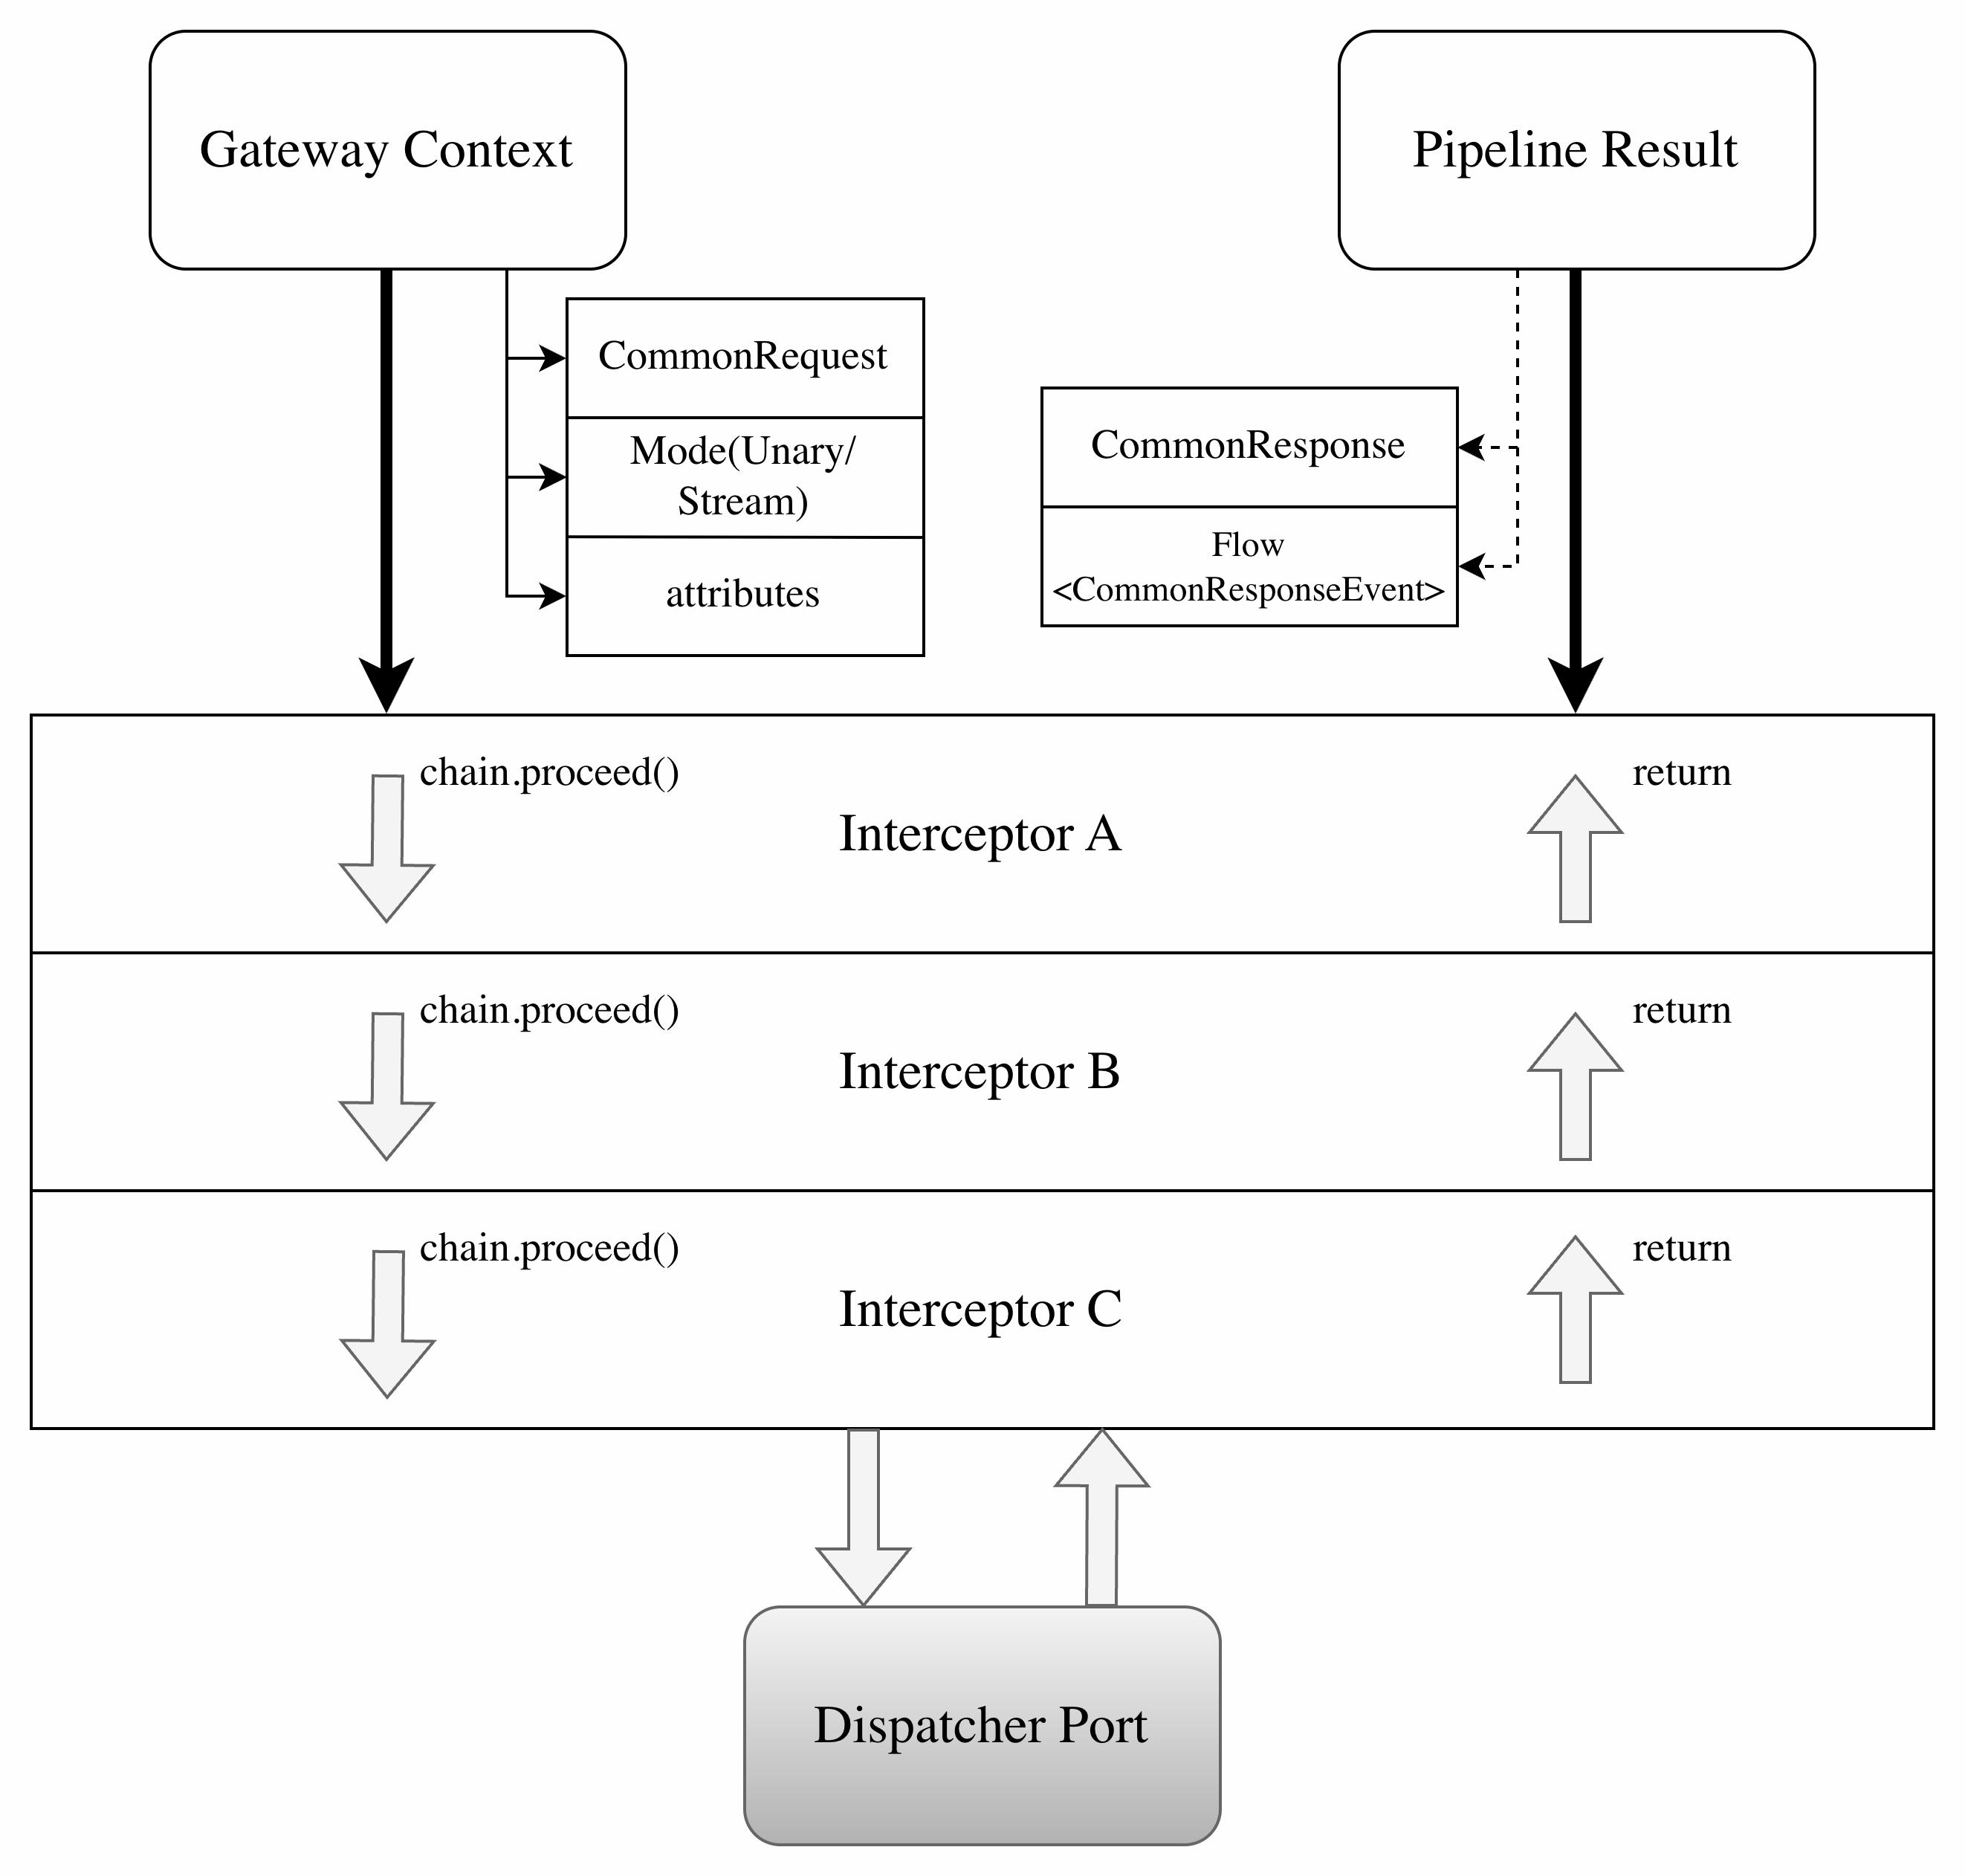
\includegraphics[width=0.9\textwidth]{../images/PipelineViewW.jpeg}
        \caption{Visão conceptual da pipeline de interceptors}
        \label{fig:pipeline}
    \end{figure}

    Esta forma de encaixe mantém a arquitetura simples. Para um caso mínimo, a Gateway pode operar com um dispatcher direto. Para um caso operacional, a pipeline permite adicionar autenticação, autorização, métricas, limites, \textit{circuit breaker}, \textit{fallback}, logging e tracing sem alterar adapters. O modelo é semelhante ao dos filtros de Servlets \cite{servlet_filterchain}: cada filtro recebe um contexto, decide se continua a cadeia e pode executar lógica antes e depois do próximo elemento. A diferença é que, no OmniAI SDK, o contexto não representa apenas um pedido HTTP; representa uma chamada de inferência já normalizada, incluindo fornecedor, modelo, modo de execução, atributos tipados e eventual fluxo de \textit{streaming}.

    A \textit{pipeline} é composta por \texttt{GatewayPipeline}, \texttt{GatewayPipelineChain}, \texttt{Interceptor} e \texttt{GatewayContext}. O \texttt{GatewayContext} transporta o pedido comum, atributos tipados e modo de execução, podendo representar chamadas síncronas ou \textit{streaming}. A cadeia executa os \textit{interceptors} por ordem e, no fim, invoca o dispatcher terminal.

    Esta abordagem também prepara o escalamento horizontal. A pipeline não exige estado global obrigatório; cada pedido transporta o seu contexto. Onde existe estado partilhável, como rate limiting ou circuit breaker, o SDK define stores substituíveis. A implementação em memória é adequada para desenvolvimento e instância única, mas pode ser trocada por Redis, base de dados ou outro backend coordenado em implantações distribuídas. Assim, várias instâncias da OmniAI Gateway podem partilhar contadores, estados de circuito e metadados operacionais sem alterar o contrato dos inbounds nem a forma como os clientes chamam a Gateway.

    \section{Arquitetura Interna dos Interceptors}
    O módulo \texttt{interceptors} inclui implementações pré-construídas para preocupações operacionais e de segurança. Todos seguem o mesmo contrato: recebem um \texttt{GatewayContext}, consultam ou acrescentam atributos à \texttt{TypedMap}, decidem se chamam \texttt{chain.proceed(context)} e podem observar ou transformar o \texttt{PipelineResult}. Esta estrutura permite colocar lógica transversal antes e depois da inferência sem acoplar essa lógica aos adapters de entrada, aos adapters de saída ou ao dispatcher.

    A ordem de execução é configurável. No target JVM, o SDK suporta a anotação \texttt{InterceptorPriority}, usada para executar primeiro interceptors com prioridade superior. No target JavaScript, onde a reflexão sobre anotações é limitada, a ordem segue a sequência definida pela DSL. Assim, autenticação e autorização podem ocorrer no início da cadeia, enquanto métricas, tracing e logging podem envolver a execução completa.

    A motivação para estes interceptors não foi apenas organizar código, mas tornar explícitas políticas que, numa Gateway de IA, afetam segurança, custo e disponibilidade. A Tabela~\ref{tab:interceptor-rationale} resume essa relação.

    \begin{table}[H]
        \centering
        \footnotesize
        \renewcommand{\arraystretch}{1.25}
        \begin{tabularx}{\textwidth}{|>{\raggedright\arraybackslash}p{3.2cm}|Y|Y|}
            \hline
            \textbf{Interceptor} & \textbf{Problema tratado} & \textbf{Motivo para estar na Gateway} \\
            \hline
            Telemetria & Falta de visibilidade sobre latência, erros, tokens e fornecedores. & A Gateway observa todas as chamadas e consegue medir comportamento transversal sem alterar clientes ou adapters. \\
            \hline
            Autenticação & Necessidade de validar quem apresenta o token antes de consumir modelos pagos. & A Gateway é o recurso protegido e deve validar tokens antes de encaminhar tráfego para fornecedores. \\
            \hline
            Autorização & Um token válido não implica permissão para todos os modelos ou operações. & A decisão por cliente, ação, fornecedor e modelo deve ser centralizada antes da inferência. \\
            \hline
            Rate limiting & Risco de abuso, picos de carga e custos inesperados. & A Gateway é o ponto natural para aplicar quotas por cliente, plano, fornecedor ou modelo. \\
            \hline
            Circuit breaker & Dependências externas podem ficar lentas ou indisponíveis. & A Gateway evita insistir em fornecedores em falha e protege o restante sistema. \\
            \hline
            Fallback & Uma falha de fornecedor não deve, quando existe alternativa, falhar imediatamente a experiência do cliente. & A Gateway conhece os outbounds disponíveis e pode tentar alternativas mantendo o contrato do cliente. \\
            \hline
        \end{tabularx}
        \caption{Justificação dos interceptors fornecidos pelo SDK}
        \label{tab:interceptor-rationale}
    \end{table}

    \subsection{Interceptor de Telemetria e Observabilidade}
    O \texttt{MetricsInterceptor} recolhe dados operacionais essenciais num sistema que intermedeia chamadas a LLMs: latência, sucesso, erro, fornecedor, modelo, cliente e consumo de tokens. Estes dados são importantes porque uma Gateway centraliza tráfego de vários clientes e fornecedores; sem telemetria, não é possível perceber custos, degradação, falhas por modelo ou impacto de políticas como \textit{fallback}.

    A implementação distingue chamadas unárias de \textit{streaming}. Em respostas progressivas, o interceptor não bloqueia a execução; usa operadores de fluxo para observar eventos e emitir métricas no encerramento do \textit{stream}. Assim mede a duração total da interação, e não apenas o tempo até ao primeiro fragmento.

    A arquitetura segue inversão de dependência através da porta \texttt{MetricsPort}. O OmniAI SDK define instrumentos comuns, como \texttt{counter}, \texttt{histogram} e \texttt{upDownCounter}, enquanto o adapter concreto no target JVM exporta para OpenTelemetry. O uso do OpenTelemetry Protocol (OTLP) foi escolhido porque o OTLP define a codificação, transporte e entrega de dados de telemetria entre fontes, coletores e backends \cite{opentelemetry_otlp}. Esta escolha evita prender o OmniAI SDK a Prometheus, Grafana, Datadog ou outro backend específico: o SDK emite telemetria num formato aberto, o Collector recebe e processa esses dados, e a infraestrutura decide para onde exportar.

    Esta decisão é especialmente importante numa Gateway de IA. O mesmo OmniAI SDK pode ser usado por uma aplicação simples em desenvolvimento, por um POC local com Prometheus/Grafana ou por uma instalação futura com outro backend de observabilidade. A OpenTelemetry apresenta-se precisamente como especificação aberta e agnóstica de fornecedor \cite{opentelemetry_what_is}; por isso, a instrumentação fica no OmniAI SDK, mas a escolha operacional do backend permanece fora do domínio.

    \begin{figure}[H]
        \centering
        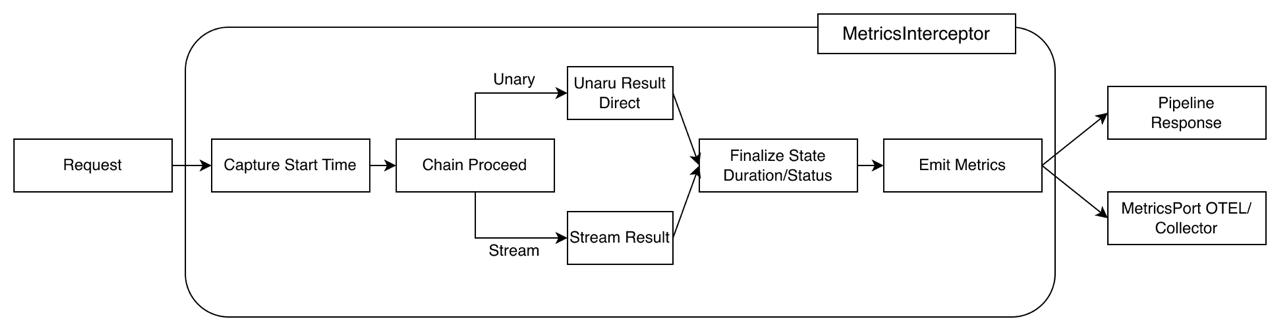
\includegraphics[width=0.9\textwidth]{../images/MetricsInterceptorArch}
        \caption{Fluxo interno de processamento e lógica de observabilidade para pedidos unários e streaming}
        \label{fig:metrics-interceptor-arch}
    \end{figure}

    Para adicionar uma métrica, a aplicação usa a DSL do \texttt{gateway-client}. O programador pode ativar a latência padrão, acrescentar atributos globais e definir métricas próprias com uma função \texttt{value}, que extrai o valor a partir do contexto e do resultado, e uma função \texttt{tags}, que acrescenta dimensões de análise.

    \begin{lstlisting}[language=kotlin, caption={Configuração de telemetria e métricas personalizadas na DSL}]
metrics {
    metricsPort = telemetryRuntime.metricsPort
    tracer = telemetryRuntime.tracer

    attributes {
        include(ClientIpMetadataKey, alias = "client.ip")
        attribute("sdk.version") { _, _ -> "1.0.0" }
    }

    defaultLatency {
        enabled = true
        name = "gateway.inference.request.duration"
    }

    customMetrics {
        counter(
            name = "gateway.llm.tokens",
            description = "Total de tokens consumidos",
            unit = "{tokens}"
        ) {
            value { _, result ->
                (result as? PipelineResult.Unary)?.response?.usage?.totalTokens
            }
        }
    }
}
    \end{lstlisting}

    Este desenho separa três responsabilidades: a definição da métrica na DSL, a recolha no interceptor e a exportação no adapter de telemetria. Também facilita testes, porque \texttt{NoOpMetricsPort} pode ser usado quando a observabilidade está desligada.

    \begin{figure}[H]
        \centering
        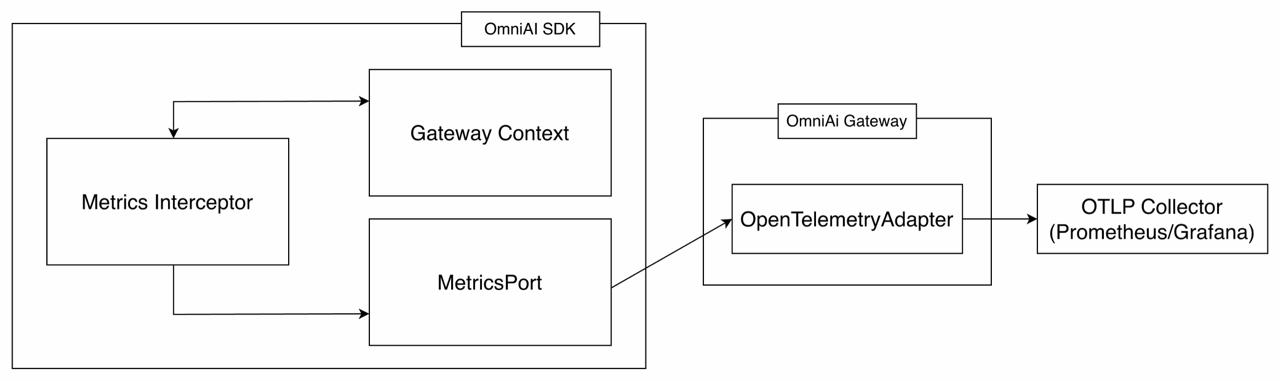
\includegraphics[width=0.9\textwidth]{../images/MetricsGateway}
        \caption{Observabilidade e métricas operacionais da OmniAI Gateway}
        \label{fig:metrics-gateway}
    \end{figure}

    \subsection{Interceptor de Autenticação}
    A autenticação é realizada pelo \texttt{AuthenticationInterceptor}. A Gateway atua como \textit{Resource Server}: recebe pedidos para recursos protegidos, extrai o \textit{access token} do cabeçalho \texttt{Authorization: Bearer <token>} e valida se esse token foi emitido por um servidor de autorização confiável \cite{rfc6749,rfc6750,oauth_resource_server}. Esta responsabilidade é essencial numa AI Gateway, porque a camada central passa a proteger acesso a modelos, custos, quotas e dados operacionais.

    A Gateway não deve atuar como \textit{Authorization Server}: não emite tokens, não gere credenciais dos clientes e não substitui Logto ou Keycloak. O seu papel é o de API protegida. Por isso, valida tokens recebidos, confirma se foram emitidos para a audiência esperada e só depois permite que o pedido avance na pipeline para os próximos interceptors Esta separação reduz responsabilidade de segurança dentro do SDK e permite integrar diferentes fornecedores de identidade sem alterar o contrato dos clientes.

    O fluxo inicia-se no adapter HTTP, que propaga o token para o domínio através de metadados. O interceptor classifica o token: se tiver três segmentos, é tratado como JWT; caso contrário, como token opaco. Esta distinção permite escolher entre validação local por assinatura e validação remota por introspeção.

    No modo \textit{OIDC Discovery} (RFC 8414), a Gateway obtém dinamicamente metadados do \textit{Authorization Server}, como \textit{issuer}, \texttt{jwks\_uri} e endpoint de introspeção \cite{rfc8414}. Todo este fluxo encontra-se ilustrado na Figura 5.4. Para JWTs, valida o \texttt{kid}, obtém a chave pública no JWKS, verifica assinatura e confirma \textit{claims} como \texttt{exp}, \texttt{nbf}, \texttt{iss} e \texttt{aud} \cite{rfc7519,rfc7517,rfc7515}. Para tokens opacos, usa introspeção OAuth2 \cite{rfc7662}.

    \begin{figure}[H]
        \centering
        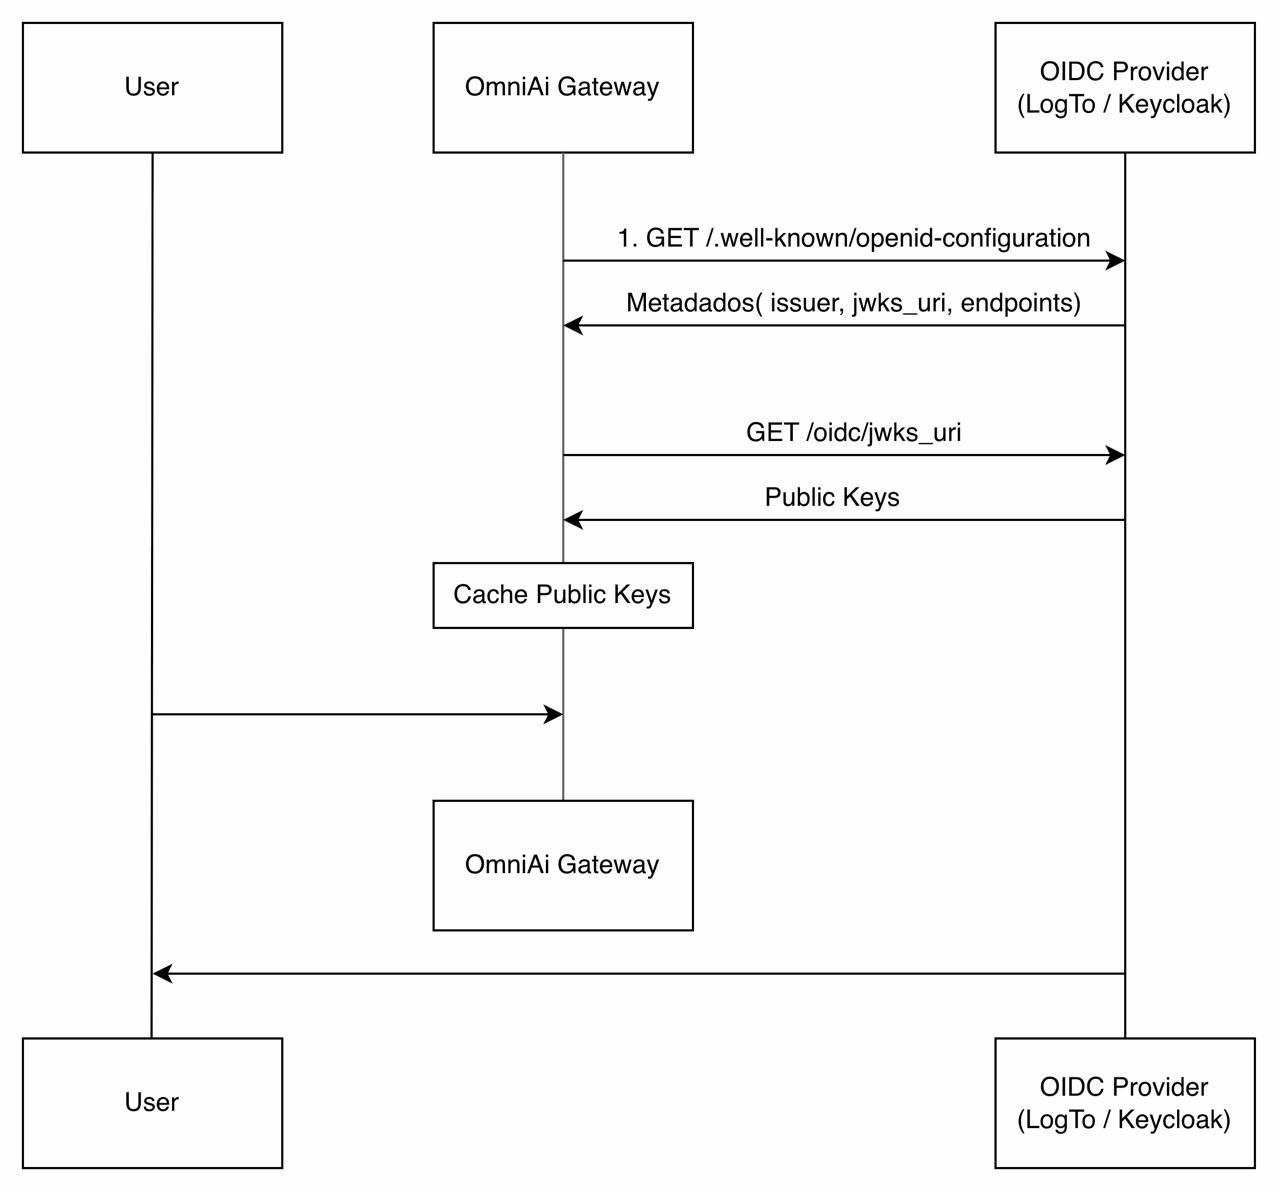
\includegraphics[width=0.9\textwidth]{../images/AutenticationFlow}
        \caption{Sequência OIDC: descoberta, JWKS e cache de chaves}
        \label{fig:oidc-sequence}
    \end{figure}

    Para reduzir latência e chamadas repetidas ao servidor de autorização, a implementação inclui \texttt{InMemoryKeyCache}, rotação de chaves em \textit{background} e \textit{cooldown} para evitar consultas excessivas quando uma chave não é encontrada. No caso de tokens opacos, o \texttt{IntrospectionCache} usa \textit{positive caching} para tokens ativos e \textit{negative caching} para tokens inválidos. Os tokens opacos são guardados em cache através de \textit{hash}, evitando manter credenciais em texto limpo em memória.

    O resultado é encapsulado em \texttt{AuthValidationResult} e guardado na \texttt{TypedMap} sob a chave \texttt{AUTH\_RESULT\_KEY}. Isto permite que autorização, métricas e logging reutilizem a identidade já validada.

    \begin{figure}[H]
        \centering
        
\includegraphics[width=\textwidth]{../images/autenticacao}
        \caption{Fluxo interno do interceptor de autenticação}
        \label{fig:auth-interceptor}
    \end{figure}

    A Gateway final usa Logto como Authorization Server local \cite{logto_docs}, executado em Docker juntamente com PostgreSQL, OpenTelemetry Collector, Prometheus e Grafana. Foram também realizados testes exploratórios com Keycloak \cite{keycloak_docs}. A escolha final do Logto no POC deveu-se à simplicidade de configuração local, suporte a aplicações Machine-to-Machine e facilidade de gerir API Resources durante a validação.

    A integração do processo de autenticação é declarada na montagem do \textit{SDK}:
    \begin{lstlisting}[language=kotlin, caption={DSL de configuração do interceptor de autenticação com OIDC Discovery}]
security {
    authentication {
        discovery {
            discoveryUrl = "https://auth.example.com/.well-known/openid-configuration"
            expectedAudience = "https://gateway.example.com/api"
            clientId = "gateway-client"
            clientSecret = "secret"
        }
    }
}
    \end{lstlisting}

    \subsection{Interceptor de Autorização}
    A autorização é separada da autenticação porque responder a ``quem é o utilizador?'' não é o mesmo que responder a ``o que este utilizador pode fazer?''. A autenticação valida identidade; a autorização decide permissões sobre uma ação e um recurso. Esta separação é importante numa Gateway multi-cliente, onde um token válido pode não ter permissão para usar todos os modelos, fornecedores ou operações. A distinção entre autenticação e autorização é também a base dos modelos modernos de identidade: a primeira prova identidade, enquanto a segunda concede permissão sobre dados ou ações protegidas \cite{microsoft_authn_authz}.

    No contexto do projeto, esta separação evita dois problemas. Primeiro, impede que a validação de token seja confundida com autorização total: um cliente autenticado pode estar limitado a um subconjunto de modelos, fornecedores ou quotas. Segundo, permite trocar a origem das decisões de autorização sem alterar a autenticação. Embora numa fase inicial a decisão possa operar de forma local e simples, o sistema está desenhado para que, numa iteração futura, essa mesma decisão possa ser assegurada por um PDP externo, tal como o AuthZen ou o OPA.

    No OmniAI SDK, a autorização é centralizada no \texttt{PolicyEnforcerInterceptor}. O componente atua como \textit{Policy Enforcement Point} (PEP): interceta o pedido, constrói um \texttt{AuthorizationInput} e delega a decisão a um \textit{Policy Decision Point} (PDP) através da porta \texttt{PolicyDecisionPointPort}.Podemos ver todo este fluxo na figura 5.6.

    \begin{figure}[H]
        \centering
        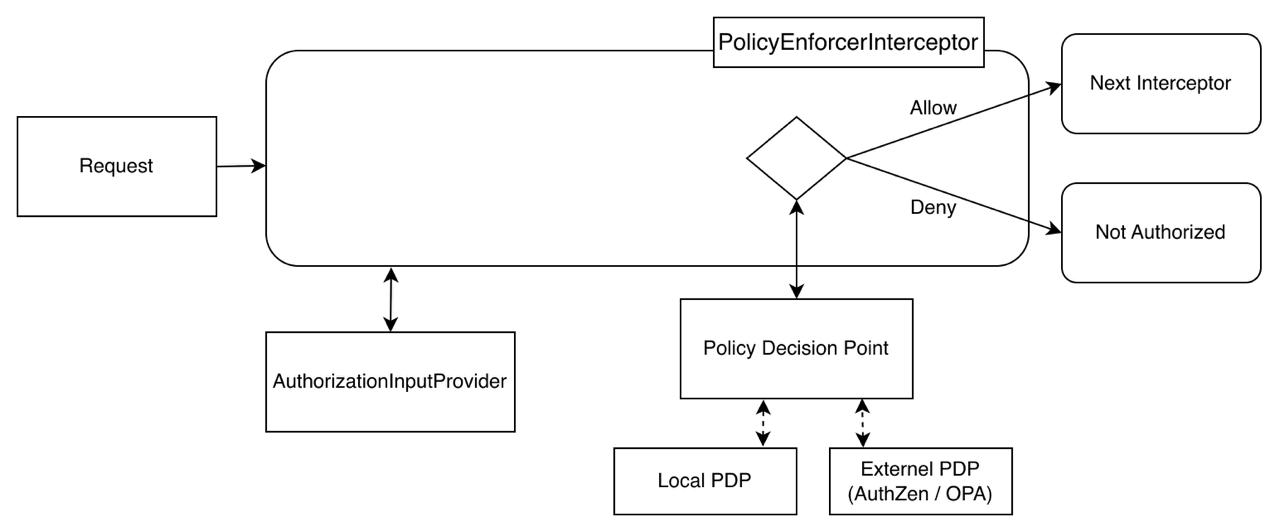
\includegraphics[width=0.9\textwidth]{../images/Authorization}
        \caption{Arquitetura do interceptor de autorização: separação entre PEP e PDP}
        \label{fig:authorization-architecture}
    \end{figure}

    O \texttt{AuthorizationInput} segue o padrão \textbf{Subject-Action-Resource (SAR)}. O \textbf{Subject} representa o utilizador ou aplicação, incluindo identificador, roles e atributos vindos do token. A \textbf{Action} representa a operação, como \texttt{chat\_completion}. O \textbf{Resource} identifica o alvo, como fornecedor ou modelo. O \textbf{Context} acrescenta atributos ambientais, como IP, tempo ou metadados do pedido. A porta do PDP permite integrar motores diferentes, incluindo políticas internas, AuthZen, OPA ou outro serviço externo. Se a decisão for \textit{Deny}, a pipeline é interrompida antes de qualquer chamada ao fornecedor \cite{authorization_pips}.

    A configuração de autorização permite estender o avaliador por omissão:
    \begin{lstlisting}[language=kotlin, caption={DSL de configuração do interceptor de autorização}]
security {
    authorization {
        pdp = customPolicyDecisionPoint
        inputProvider = DefaultAuthorizationInputProvider
    }
}
    \end{lstlisting}

    \subsection{Interceptor de Rate Limiting}
    O \texttt{RateLimitInterceptor} aplica limites de utilização antes da chamada ao fornecedor. Numa AI Gateway, este mecanismo tem dois objetivos principais: proteger o sistema contra abuso ou tráfego excessivo e controlar custos associados a chamadas de inferência. A limitação de taxa é uma estratégia comum para impor um teto de ações repetidas num intervalo temporal, reduzindo abuso de APIs, força bruta e carga excessiva \cite{cloudflare_rate_limiting}.

    A importância deste interceptor é maior do que numa API tradicional, porque cada pedido pode representar custo financeiro direto, consumo de quotas externas e ocupação prolongada de ligações em \textit{streaming}. Sem rate limiting, um cliente mal configurado, uma automação em ciclo ou um utilizador abusivo pode saturar a Gateway, esgotar quotas nos fornecedores e degradar o serviço para clientes legítimos. O interceptor permite aplicar justiça operacional: cada cliente, plano, modelo ou fornecedor pode ter limites próprios.

    A lógica é orientada por políticas. Cada \texttt{RateLimitPolicy} extrai dados do \texttt{GatewayContext} e devolve \texttt{RateLimitTarget}. Um target contém uma chave, como cliente/modelo/plano, e uma \texttt{RateLimitDefinition}, composta por limite, tipo e janela temporal. Isto permite políticas diferentes por cliente, plano, modelo ou fornecedor.

    O store atual em memória usa buckets protegidos por \texttt{Mutex}. Quando um pedido chega, o interceptor tenta consumir uma unidade em todos os buckets aplicáveis. Se todos permitirem consumo, a cadeia continua. Se algum limite estiver esgotado, devolve \texttt{TooManyRequestsError} com \texttt{retryAfter}. Esta resposta permite que clientes bem comportados reduzam ritmo em vez de insistirem. Para desenvolvimento e instância única, este modelo é suficiente; em escalamento horizontal, o contrato \texttt{RateLimitStore} permite substituir a implementação por Redis ou outro backend partilhado. Essa substituição é necessária quando várias instâncias da Gateway devem partilhar a mesma visão de quota.

    A configuração deste mecanismo recorre ao seguinte bloco:
    \begin{lstlisting}[language=kotlin, caption={DSL de configuração do interceptor de rate limiting}]
interceptors {
    rateLimiting {
        store = InMemoryRateLimitStore()
        addPolicy(rateLimitPolicy)
    }
}
    \end{lstlisting}

    \subsection{Interceptor de Circuit Breaker}
    O \texttt{CircuitBreakerInterceptor} protege a Gateway contra chamadas repetidas a um outbound em falha. O padrão de \textit{circuit breaker} é usado para lidar com falhas em serviços remotos, evitando insistir numa dependência que está indisponível e dando tempo para recuperação \cite{microsoft_circuit_breaker,itau_circuit_breaker,treinaweb_circuit_breaker}. Numa Gateway de IA, esta proteção é especialmente útil porque fornecedores externos podem falhar por indisponibilidade, timeouts, quotas ou erros 5xx.

    A alternativa simples seria repetir pedidos até obter sucesso. Essa abordagem é perigosa quando o fornecedor está realmente indisponível: as tentativas acumulam latência, ocupam threads ou corrotinas, aumentam custos e podem agravar a falha no serviço externo. O circuit breaker foi criado para evitar esse comportamento. Quando a falha ultrapassa um limiar, o circuito abre e a Gateway passa a falhar rapidamente aquele destino, libertando recursos e permitindo que mecanismos como fallback escolham outro outbound.

    Para cada combinação de fornecedor/modelo, o interceptor identifica o \texttt{outbound.key} e consulta o \texttt{CircuitBreakerStore}. Se o circuito estiver \texttt{OPEN}, o pedido falha rapidamente com \texttt{ApiDownError} e o outbound é acrescentado ao conjunto de outbounds negados no contexto. Esta falha rápida reduz latência, evita consumo de recursos e dá ao \textit{fallback} informação para não tentar novamente o mesmo destino.

    Quando a chamada prossegue, o interceptor observa o resultado. Erros incrementam o contador de falhas; ao atingir \texttt{failureThreshold}, o circuito passa para \texttt{OPEN}. Após um período de recuperação, o estado \texttt{HALF\_OPEN} permite testar um número limitado de pedidos antes de voltar ao estado \texttt{CLOSED}, evitando inundar um fornecedor que ainda está a recuperar \cite{microsoft_circuit_breaker}. A configuração inclui \texttt{failureThreshold}, \texttt{resetTimeoutMs} e \texttt{halfOpenTestRequests}. A implementação atual cobre a abertura e fecho básico do circuito; a evolução temporal mais completa do estado \texttt{HALF\_OPEN} é uma melhoria natural.

    \begin{lstlisting}[language=kotlin, caption={DSL de configuração do interceptor de circuit breaker}]
interceptors {
    circuitBreaker {
        store = InMemoryCircuitBreakerStore()
        config = CircuitBreakerConfig(
            failureThreshold = 5,
            resetTimeoutMs = 10000L,
            halfOpenTestRequests = 2
        )
    }
}
    \end{lstlisting}

    \subsection{Interceptor de Fallback}
    O \texttt{FallbackInterceptor} permite tentar alternativas quando a chamada principal falha. Em sistemas de IA, \textit{fallback} ao nível de modelo ou fornecedor é relevante porque falhas nas APIs de inferência fornecidas pelas LLM's são um cenário frequente em produção: rate limits, indisponibilidade, quotas, timeouts ou modelos descontinuados podem impedir a resposta do fornecedor principal \cite{ai_fallback_tombas,portkey_fallback}. Um gateway é o ponto certo para esta política, porque conhece os outbounds configurados e consegue trocar de destino sem exigir alterações no cliente.

    A decisão de colocar fallback na Gateway, e não nos clientes, reduz duplicação e melhora controlo operacional. Se cada aplicação cliente implementasse a sua própria lógica de fallback, seria necessário repetir regras de prioridade, tratamento de erros, mapeamento de contratos e métricas em vários pontos. Ao centralizar a política, o SDK consegue manter o mesmo contrato de entrada e decidir internamente que fornecedor ou modelo alternativo deve ser tentado. Isto é particularmente útil quando o cliente usa um contrato compatível com Anthropic ou OpenAI, mas a Gateway pode executar a chamada noutro provider configurado.

    A implementação atual usa a lista de outbounds disponíveis. Primeiro tenta o outbound correspondente ao fornecedor e modelo pedidos; se falhar, acrescenta esse outbound ao conjunto de negados e tenta alternativas. Para cada tentativa, cria um novo \texttt{GatewayContext} com os mesmos atributos, mas com \texttt{provider} e \texttt{model} atualizados para o outbound alternativo.

    A integração com o circuit breaker é feita através do conjunto partilhado de outbounds negados. Assim, se um circuito estiver aberto, o fallback evita esse destino e tenta outro modelo ou fornecedor. Este desenho permite construir políticas de resiliência como ``tentar Gemini, depois OpenAI-compatible via Groq, depois Anthropic'', mantendo a lógica de tentativa fora dos adapters. Também permite distinguir degradação controlada de erro total: a resposta pode chegar por um modelo alternativo, enquanto métricas e tracing registam que ocorreu fallback.

    A evolução futura poderá acrescentar prioridades configuráveis, condições por código de erro, orçamentos de tentativa e métricas específicas de fallback. Estas regras são importantes porque nem todo erro justifica fallback: erros de autenticação ou autorização devem falhar imediatamente, enquanto timeouts, 429 e 5xx podem justificar uma alternativa.

    A sua ativação é extremamente simples, não requerendo configuração intrincada:
    \begin{lstlisting}[language=kotlin, caption={DSL de configuração do interceptor de fallback}]
interceptors {
    fallback()
}
    \end{lstlisting}

    \subsection{Interceptor de Logging e Tracing}
    O \texttt{RequestLoggingInterceptor} regista fornecedor, modelo, sucesso, erro e conclusão de streams através da abstração \texttt{GatewayLogger}. No target JVM pode ser ligado a SLF4J; no target JavaScript pode usar consola ou outra integração. O objetivo é garantir visibilidade mínima mesmo quando a telemetria completa não está ativa.

    O logging foi mantido separado das métricas porque responde a perguntas diferentes. Métricas mostram tendências agregadas, como latência média ou número de erros; logs ajudam a explicar um pedido concreto. Numa Gateway de IA, esta distinção também tem impacto de privacidade: o objetivo é registar metadados operacionais, e não despejar prompts, respostas completas ou tokens sensíveis nos logs.

    O \texttt{TracingInterceptor} envolve o pedido num \textit{span} chamado \texttt{gateway.request.process}. Quando combinado com OpenTelemetry, este span permite correlacionar latência, erros, chamadas externas e métricas agregadas. Em cenários de fallback ou circuit breaker, tracing é particularmente útil porque permite observar o percurso real do pedido e distinguir falhas do fornecedor, decisões da Gateway e erros de cliente. Também permite perceber se uma resposta lenta resulta do fornecedor principal, de uma tentativa alternativa, de validação de token ou de uma política interna.

    A instalação processa-se em dois blocos da DSL, um explícito e outro decorrente da configuração de métricas:
    \begin{lstlisting}[language=kotlin, caption={Instalação dos interceptors de logging e tracing}]
interceptors {
    // Instalacao manual do Logging Interceptor
    use(RequestLoggingInterceptor(logger))
    
    // O TracingInterceptor e instalado automaticamente ao fornecer o tracer as metricas
    metrics {
        tracer = telemetryRuntime.tracer
    }
}
    \end{lstlisting}

    \section{MCP Broker e Ferramentas Externas}

    O MCP Broker foi introduzido como consequência do estudo do MCP e do \textit{tool calling}. O objetivo é separar a gestão de ferramentas externas da lógica específica das APIs de inferência. Em vez de cada adapter conhecer diretamente as ferramentas disponíveis e a forma como são executadas, o broker fornece uma camada intermédia para representar ferramentas, recursos e \textit{prompts} de forma uniforme.

    O módulo \texttt{mcp-broker} depende da biblioteca \texttt{io.modelcontextprotocol:kotlin-sdk}. A implementação atual inclui modelos para ferramentas, recursos e \textit{prompts}, geração de esquemas JSON, configuração de transportes \texttt{stdio}, SSE e WebSocket, e mapeamento entre o domínio do projeto e tipos do SDK MCP. A classe \texttt{McpTool} descreve uma ferramenta por nome, descrição, serializer e função \texttt{execute}; \texttt{McpServerBuilder} permite registar ferramentas, recursos e \textit{prompts} de forma declarativa.

    A Figura~\ref{fig:tool-calling} representa o ciclo geral de \textit{tool calling}. Primeiro, o cliente envia um pedido com ferramentas disponíveis. Em seguida, o modelo pode pedir uma chamada estruturada com nome e argumentos. A aplicação executa ou encaminha a ferramenta, devolve o resultado ao modelo e recebe a resposta final. O MCP Broker foi desenhado para suportar esta separação no futuro, permitindo que ferramentas sejam registadas e disponibilizadas sem acoplar cada adapter de inferência ao conjunto concreto de ferramentas.

    \begin{figure}[H]
        \centering
        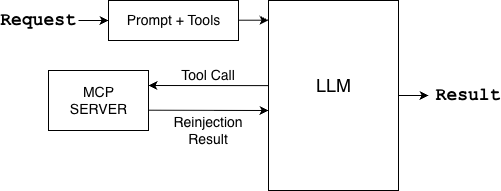
\includegraphics[width=0.45\textwidth]{../images/ToolCallingCycle}
        \caption{Representação do ciclo de \textit{tool calling} e interação com ferramentas externas}
        \label{fig:tool-calling}
    \end{figure}

    No estado atual, o módulo estabelece sobretudo as abstrações, os modelos e o mapeamento necessários para essa evolução. A execução completa de ferramentas via MCP Broker, o carregamento por YAML e a integração no POC OmniAI Gateway permanecem como trabalho futuro. Esta delimitação é importante: o POC valida contratos HTTP, autenticação, telemetria e consumo do SDK, mas ainda não demonstra invocação real via MCP Broker.

    \section{Distribuição Multiplataforma}

    Um dos objetivos do OmniAI SDK é permitir que a lógica principal da Gateway seja reutilizada em diferentes ambientes de execução. O Kotlin Multiplatform permite separar código comum de implementações específicas: o domínio, contratos, portas, adapters principais, DSL e parte dos interceptors vivem em source sets comuns; detalhes como cliente HTTP, reflexão de prioridades, servidor Ktor e integrações de plataforma ficam em source sets específicos.

    No target JVM, o OmniAI-SDK pode ser utilizado por aplicações Kotlin ou Java. Este é o target mais consolidado no estado atual do projeto e é o usado pelo POC OmniAI Gateway. A implementação JVM inclui Ktor HTTP client, integração com servidor Ktor, autenticação com descoberta OIDC, telemetria e execução real de outbounds. A distribuição futura via Maven permitirá que uma aplicação adicione o SDK como dependência versionada, sem depender de \textit{composite build}.

    No target JavaScript/Node.js, o projeto prepara uma API consumível a partir do ecossistema Node.js e TypeScript. A fachada \texttt{@JsExport} encapsula a configuração em tipos exportáveis e evita expor diretamente estruturas Kotlin que não são adequadas à fronteira JS. Esta camada é uma base para consumo via NPM, mas ainda não tem paridade total com a JVM.

    A nuance principal da distribuição multiplataforma é que nem tudo deve ser comum. O domínio e os contratos devem permanecer partilhados; transporte HTTP, servidor, observabilidade e segurança podem ter implementações diferentes por plataforma. Esta divisão evita duplicação sem forçar uma abstração demasiado rígida. A linha de evolução prevista é consolidar a API pública do OmniAI-SDK, estabilizar versionamento semântico, automatizar publicação Maven/NPM por CD e documentar exemplos mínimos de consumo para JVM e Node.js.

